\documentclass[11pt,a4paper]{article}
\usepackage[T1]{fontenc}
\usepackage{lmodern}
\usepackage[margin=2.2cm]{geometry}
\usepackage{graphicx}
\usepackage{float}
\usepackage{caption}
\captionsetup{font=small,labelfont=bf}
\setlength{\parskip}{0.5em}
\setlength{\parindent}{0pt}
\usepackage[hidelinks,bookmarksnumbered]{hyperref}

\title{S\&P 500 market analysis}
\author{Data as of 2026-10-31; 9 GICS sectors}
\date{}
\begin{document}
\maketitle
\begin{abstract}
This report describes the market data behind the value-investing and machine-learning tools: company fundamentals from SEC EDGAR filings, prices and dividends from Yahoo Finance, and the USD/ZAR exchange rate from FRED. It moves from coarse to fine: the GICS sectors against the S\&P 500, then for each analysis all sectors side by side, its best and worst sector, and the best and worst companies of those two sectors; every sector's companies are in the appendix. Companies are the current S\&P 500 members outside the Financials and Real Estate sectors; those that left the index are not included, so the results carry survivorship bias. All returns include reinvested dividends and all amounts are in US dollars.
\end{abstract}
\tableofcontents
\newpage
\section{Introduction}
\label{sec:introduction}
\begin{center}
\small
\begin{tabular}{p{3.4cm}p{8.6cm}rl}
\hline
GICS sector & What it covers & Companies & Fund \\
\hline
Communication Services & Telecommunication carriers, media, entertainment and interactive online platforms. & 22 & XLC \\
Consumer Discretionary & Goods and services households buy by choice: cars, retail, hotels, restaurants, leisure. & 47 & XLY \\
Consumer Staples & Goods households need regardless of the economy: food, beverages, tobacco, household products. & 34 & XLP \\
Energy & Oil, gas and coal: exploration, production, refining, and energy equipment and services. & 21 & XLE \\
Health Care & Pharmaceuticals, biotechnology, medical equipment and health-care providers. & 60 & XLV \\
Industrials & Capital goods, aerospace and defence, transport, and commercial and professional services. & 83 & XLI \\
Information Technology & Software, IT services, hardware, semiconductors and electronic equipment. & 75 & XLK \\
Materials & Chemicals, construction materials, containers and packaging, metals and mining. & 24 & XLB \\
Utilities & Electric, gas and water utilities and independent power producers. & 31 & XLU \\
\hline
\end{tabular}
\end{center}
Companies are grouped by the Global Industry Classification Standard (GICS), which S\&P and MSCI use to classify every listed company by its principal business. The analysis uses the eleven GICS sectors, the top level of the classification; Financials and Real Estate are left out of the stock universe because the balance-sheet rules of value investing do not fit banks, insurers and real-estate trusts. Each sector is compared with its SPDR sector fund, which tracks the S\&P 500 sector index and includes dividends, and with the S\&P 500 total-return index. The table lists the sectors analysed, the number of their companies with prices, and their fund.

\section{Overview: sectors against the S\&P 500}
\label{sec:overview}
Each GICS sector is represented by its sector fund, the market by the S\&P 500 total-return index; both include reinvested dividends. Relative return divides a fund's growth by the S\&P 500's growth over the same period, so a value above one means the sector beat the market since the start.

\begin{figure}[H]
\centering
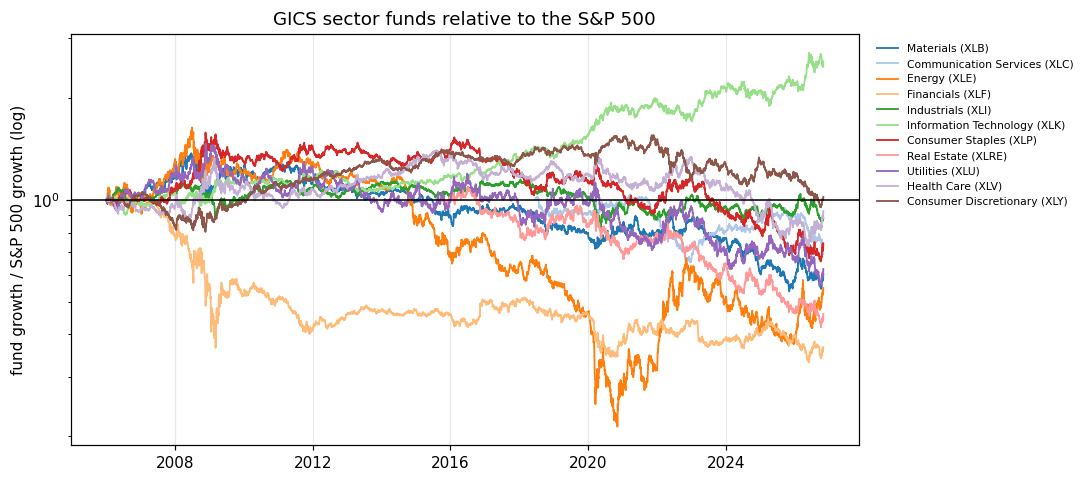
\includegraphics[width=\textwidth]{overview/relative.png}
\caption{GICS sector funds relative to the S\&P 500 total-return index, log scale; above 1 the sector outperformed the market since 2006 (or since the fund's first date).}
\end{figure}
\begin{figure}[H]
\centering
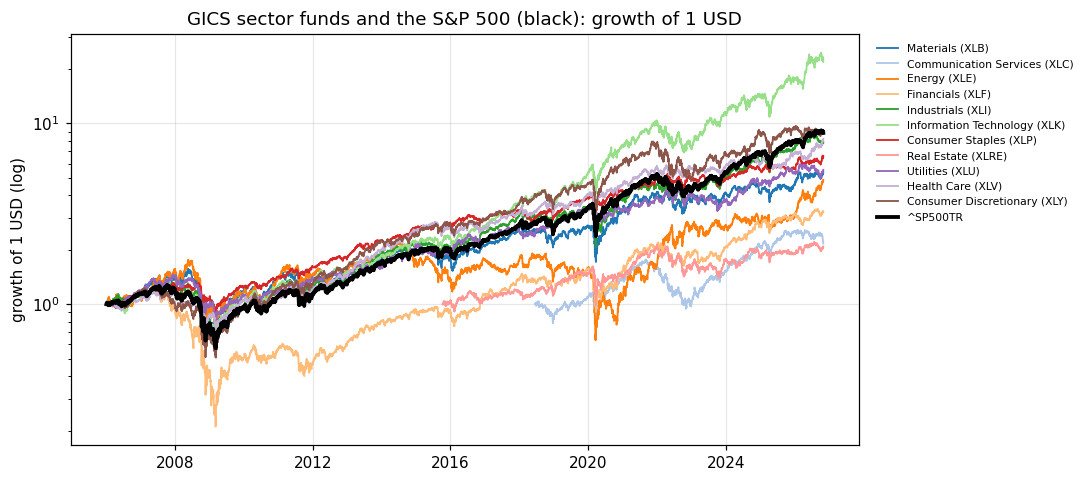
\includegraphics[width=\textwidth]{overview/total.png}
\caption{Growth of 1 USD with dividends reinvested for each GICS sector fund and the S\&P 500 (black), log scale.}
\end{figure}
\section{Fundamentals: revenue and net income}
\label{sec:fundamentals}
Revenue and net income are the values first reported in each company's annual report (10-K), in millions of US dollars, as filed with the SEC; later restatements are not used. Sector totals sum the companies of a sector per fiscal year and move when the number of reporting companies changes, especially before 2009. The fiscal year of the data date is left out, as it is not complete. A company's score is its annualised revenue growth, $g = (V_T / V_0)^{1/Y} - 1$ over at least three years; a sector's score is the median of its companies' scores, and the highest is best.

\begin{figure}[H]
\centering
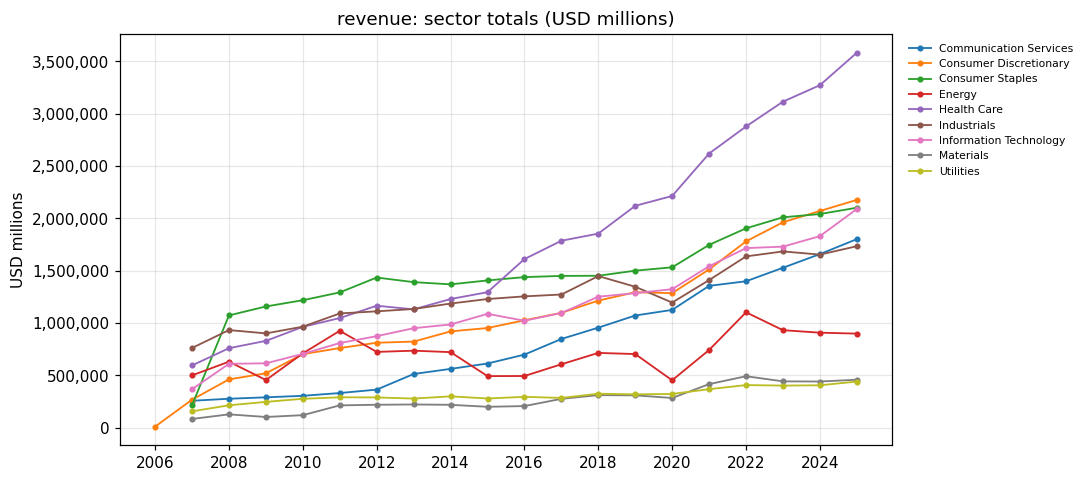
\includegraphics[width=\textwidth]{fundamentals/revenue.png}
\caption{Sum of first-reported annual revenue per GICS sector, USD millions.}
\end{figure}
\begin{figure}[H]
\centering
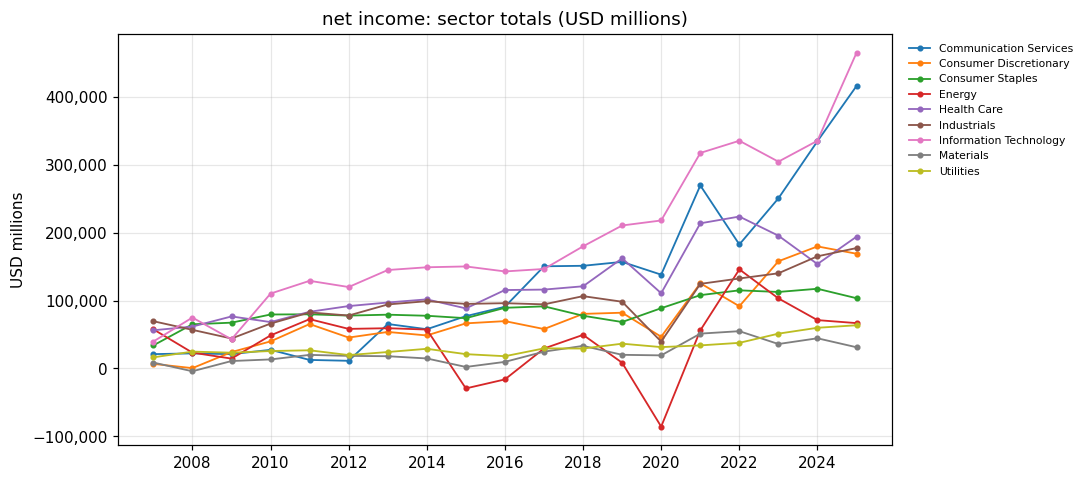
\includegraphics[width=\textwidth]{fundamentals/net_income.png}
\caption{Sum of first-reported annual net income per GICS sector, USD millions; negative values are sector-wide losses.}
\end{figure}
\subsection{Best and worst sector}
By median annualised revenue growth, Communication Services ranks first (11.9\% a year) and Utilities last (2.3\% a year). Every sector is shown in Appendix \ref{app:fundamentals}.

\begin{figure}[H]
\centering
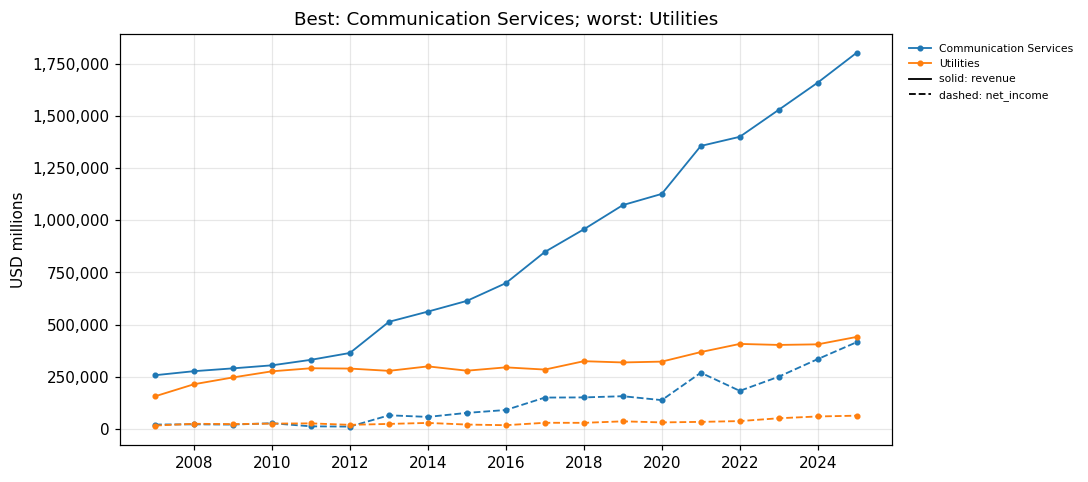
\includegraphics[width=\textwidth]{fundamentals/sectors.png}
\caption{Total revenue (solid) and net income (dashed) of Communication Services, the sector with the highest median revenue growth (11.9\% a year), and Utilities, the lowest (2.3\% a year); USD millions.}
\end{figure}
\subsection{Companies in Communication Services and Utilities}
Within each of the two sectors, the five companies with the highest revenue growth against the five with the lowest.

\begin{figure}[H]
\centering
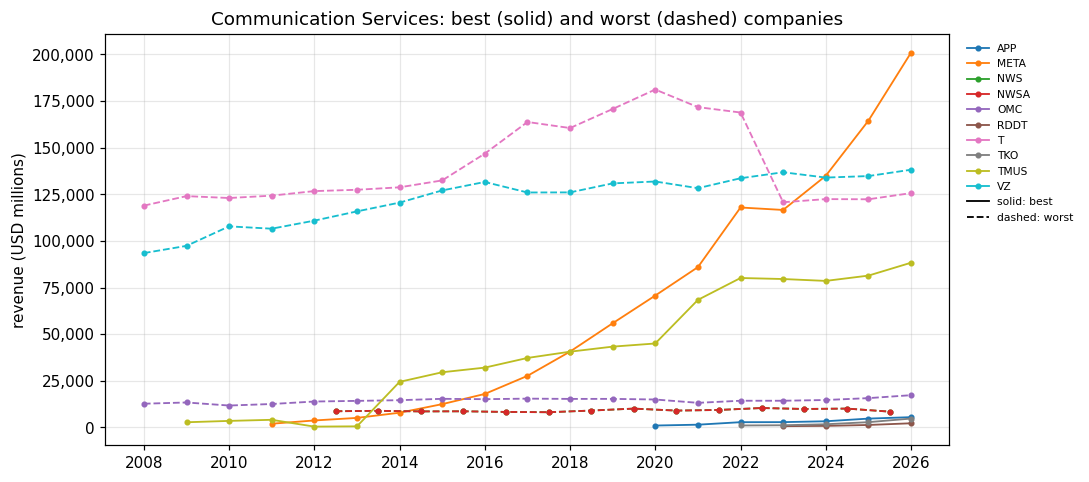
\includegraphics[width=\textwidth]{fundamentals/companies_best.png}
\caption{Communication Services: revenue of the 5 companies with the highest (solid) and lowest (dashed) annualised revenue growth, USD millions.}
\end{figure}
\begin{figure}[H]
\centering
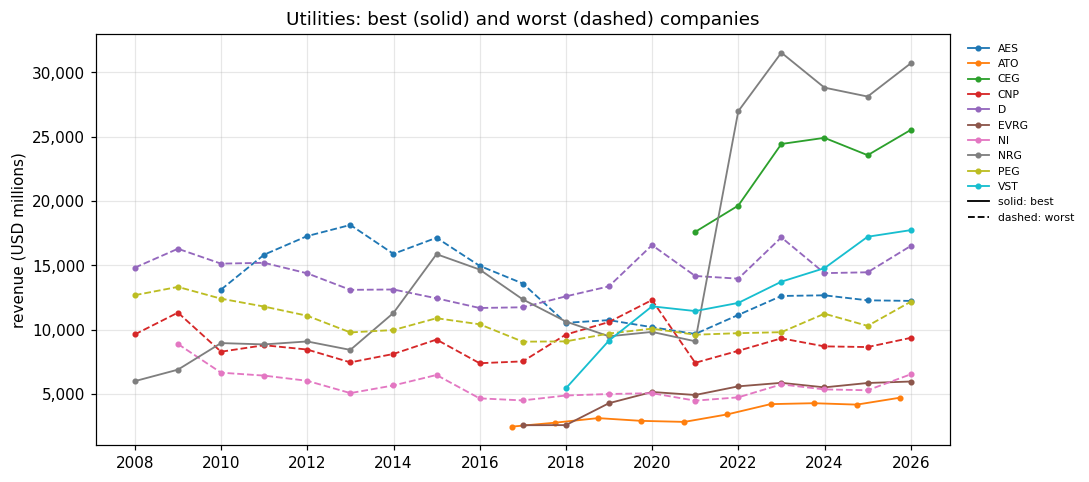
\includegraphics[width=\textwidth]{fundamentals/companies_worst.png}
\caption{Utilities: revenue of the 5 companies with the highest (solid) and lowest (dashed) annualised revenue growth, USD millions.}
\end{figure}
\section{Total return}
\label{sec:total_return}
Growth of one US dollar invested with dividends reinvested, from each series' first trading day in the data (2006 at the earliest). A company's score is its annualised total return $r = (P_T / P_0)^{1/Y} - 1$, with $P$ the dividend-adjusted price and $Y$ the years in the data (at least one); a sector's score is that of its fund, and the highest is best. All sectors are shown in the overview.

\subsection{Best and worst sector}
Information Technology returned the most (16.0\% a year) and Energy the least (7.9\% a year). Every sector's companies are in Appendix \ref{app:total_return}.

\begin{figure}[H]
\centering
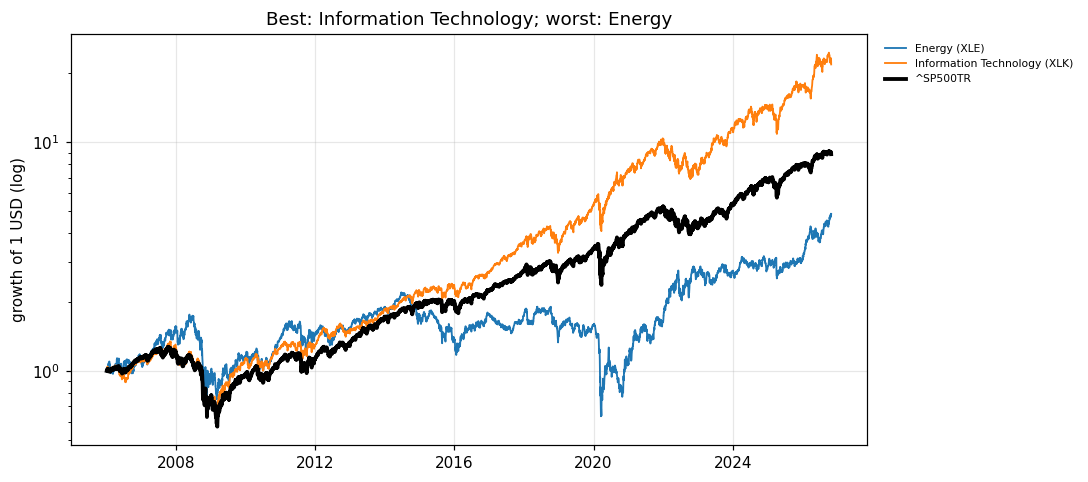
\includegraphics[width=\textwidth]{total_return/sectors.png}
\caption{Growth of 1 USD for the funds of Information Technology, the sector with the highest annualised return (16.0\% a year), and Energy, the lowest (7.9\% a year), with the S\&P 500 in black; log scale.}
\end{figure}
\subsection{Companies in Information Technology and Energy}
Within each of the two sectors, the five companies with the highest total return against the five with the lowest.

\begin{figure}[H]
\centering
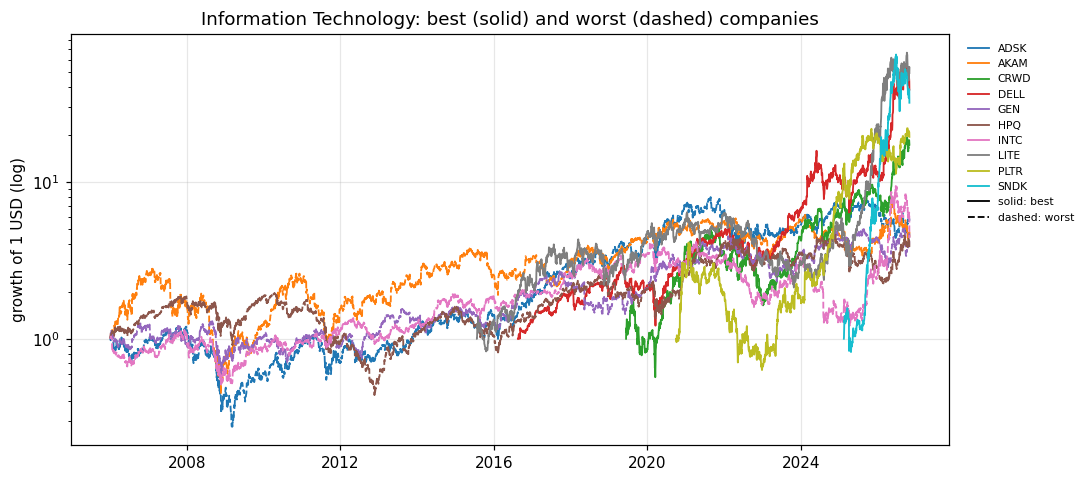
\includegraphics[width=\textwidth]{total_return/companies_best.png}
\caption{Information Technology: growth of 1 USD for the 5 companies with the highest (solid) and lowest (dashed) annualised total return, log scale.}
\end{figure}
\begin{figure}[H]
\centering
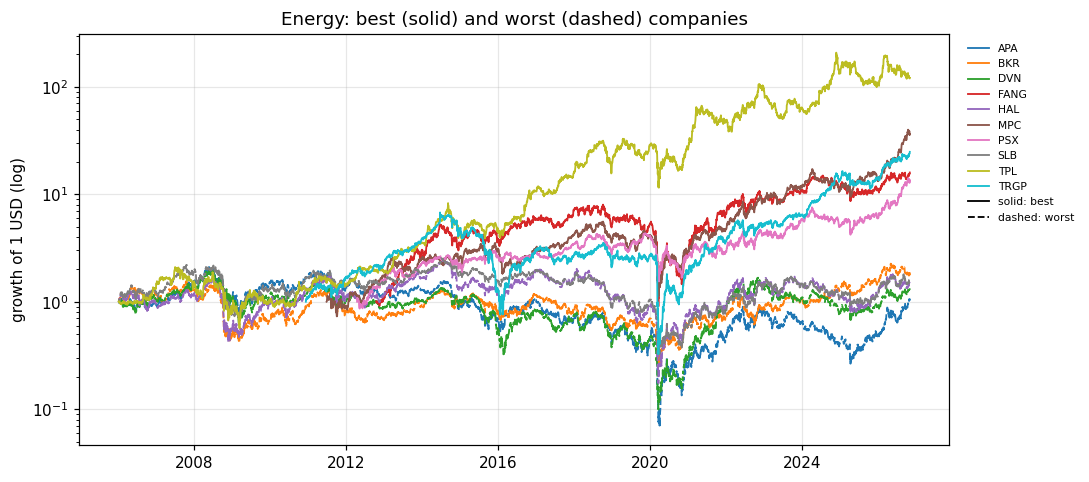
\includegraphics[width=\textwidth]{total_return/companies_worst.png}
\caption{Energy: growth of 1 USD for the 5 companies with the highest (solid) and lowest (dashed) annualised total return, log scale.}
\end{figure}
\section{Relative return}
\label{sec:relative_return}
A series' growth divided by a benchmark's growth over the same period. Sectors are compared with the S\&P 500 and companies with their sector fund, separating performance within the sector from performance of the sector. Scores are annualised relative returns, $r = G^{1/Y} - 1$, where $G$ is the relative growth and $Y$ the years (at least one); the highest is best.

\subsection{Best and worst sector}
Against the S\&P 500, Information Technology did best (4.4\% a year) and Communication Services worst (-4.3\% a year). Every sector's companies are in Appendix \ref{app:relative_return}.

\begin{figure}[H]
\centering
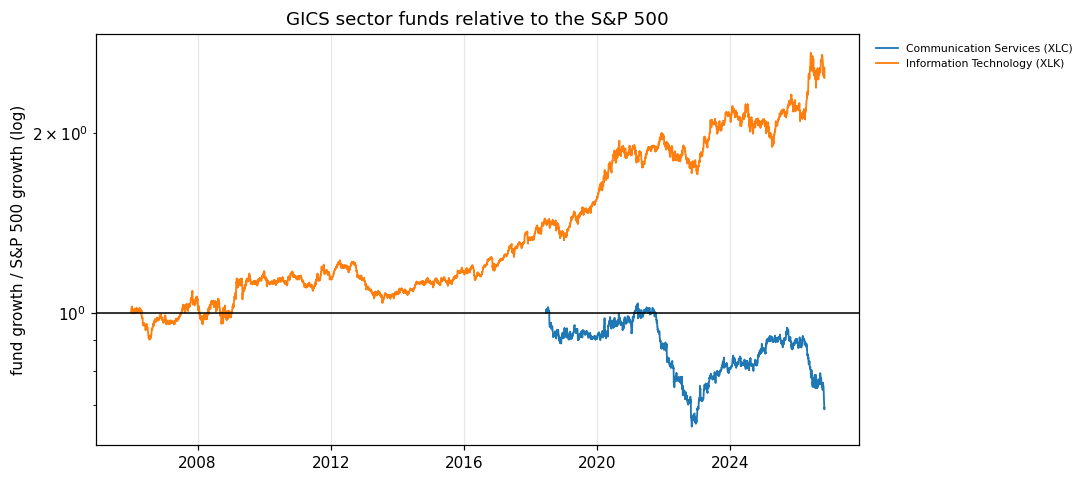
\includegraphics[width=\textwidth]{relative_return/sectors.png}
\caption{Funds of Information Technology (best, 4.4\% a year against the S\&P 500) and Communication Services (worst, -4.3\% a year), relative to the S\&P 500; log scale, above 1 the sector outperformed.}
\end{figure}
\subsection{Companies in Information Technology and Communication Services}
Within each of the two sectors, the five companies that beat their sector fund by the most against the five that trailed it by the most.

\begin{figure}[H]
\centering
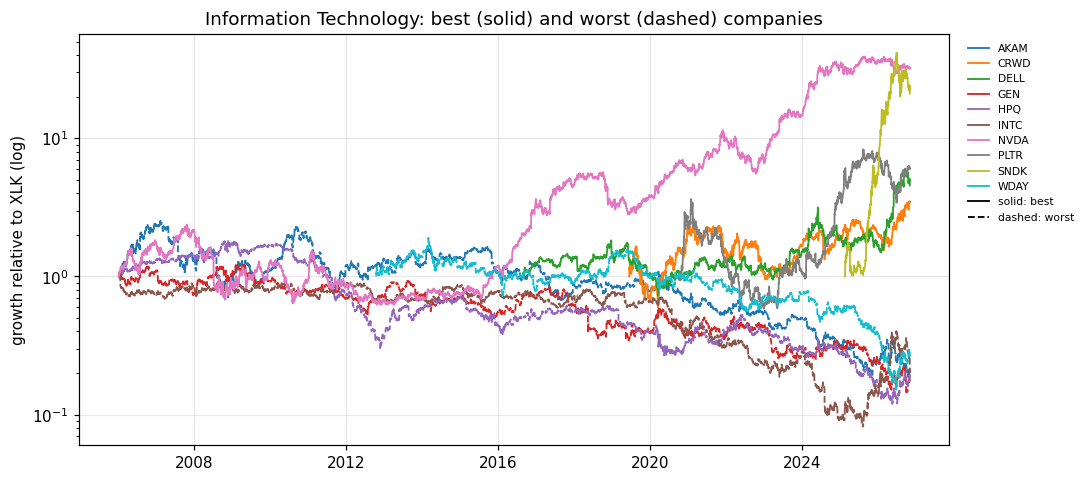
\includegraphics[width=\textwidth]{relative_return/companies_best.png}
\caption{Information Technology: the 5 companies with the highest (solid) and lowest (dashed) annualised return relative to XLK, shown as growth relative to XLK; log scale.}
\end{figure}
\begin{figure}[H]
\centering
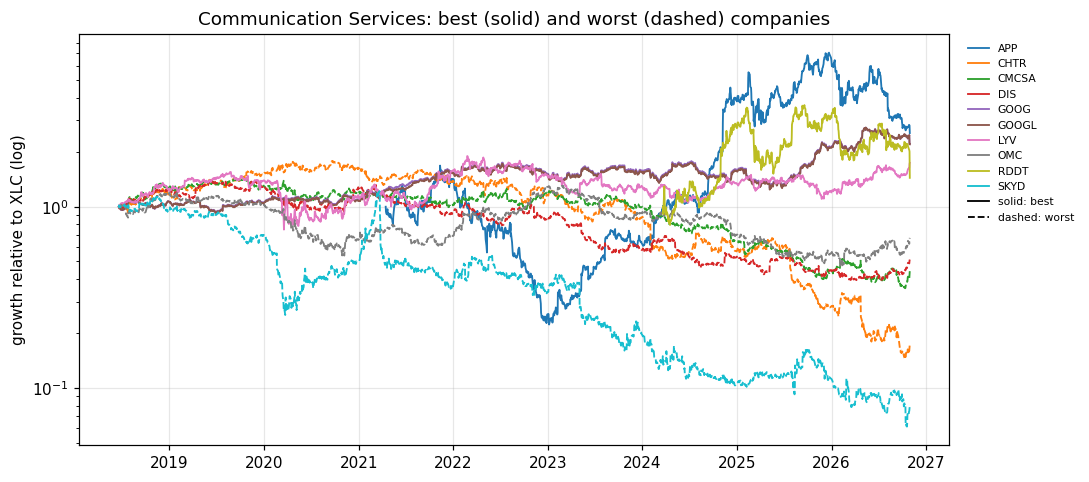
\includegraphics[width=\textwidth]{relative_return/companies_worst.png}
\caption{Communication Services: the 5 companies with the highest (solid) and lowest (dashed) annualised return relative to XLC, shown as growth relative to XLC; log scale.}
\end{figure}
\section{Price-to-earnings ratio}
\label{sec:pe}
The P/E divides the share price by the latest first-reported annual diluted earnings per share filed before the day, with EPS put on the price's split basis. It changes in steps once a year, when a new annual report is filed; a ratio on trailing twelve-month earnings will replace it. Companies with zero or negative earnings have no P/E. A company's score is its median P/E over the data; a sector's score is the median of its companies', and the lowest is best, as value investing looks for cheap earnings. The P/E of a sector is shown with the price growth of its companies, each with the band from the 25th to the 75th percentile, to show how the two move together.

\begin{figure}[H]
\centering
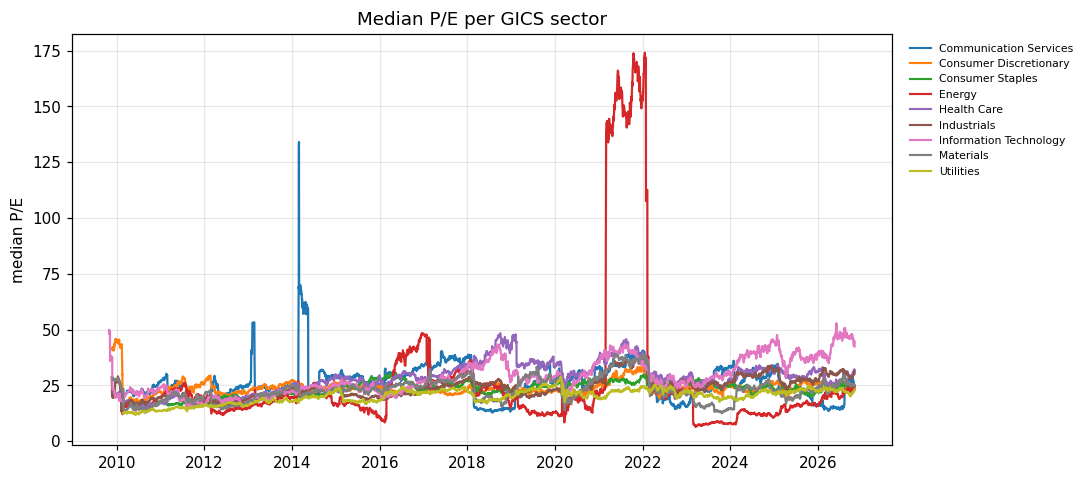
\includegraphics[width=\textwidth]{pe/summary.png}
\caption{Median P/E of the companies in each GICS sector.}
\end{figure}
\begin{figure}[H]
\centering
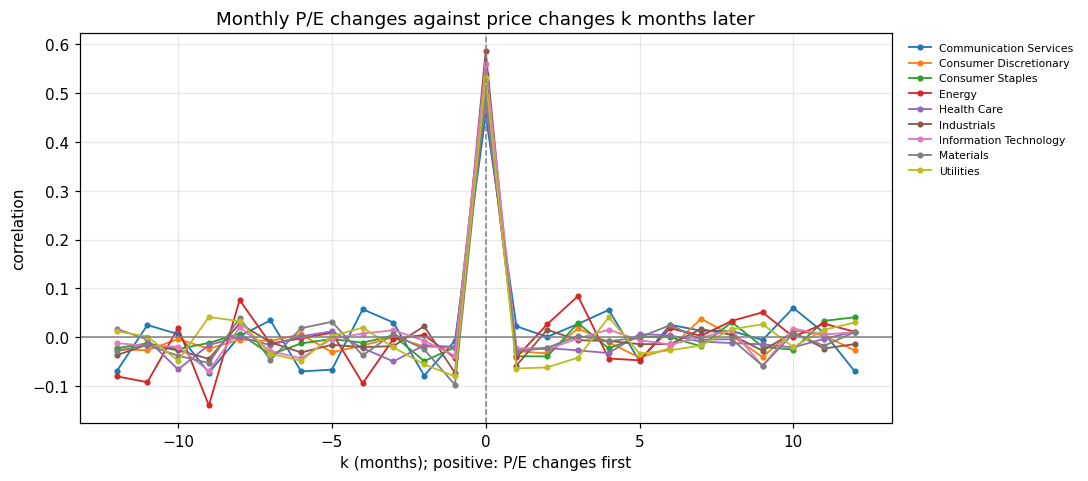
\includegraphics[width=\textwidth]{pe/lead_lag.png}
\caption{Mean correlation, over each sector's companies, of monthly P/E changes with price changes k months later; positive k: the P/E changes first.}
\end{figure}
\subsection{P/E against value: best and worst P/E}
Energy has the lowest median P/E (15.0) and Communication Services the highest (34.9). Every sector's companies are in Appendix \ref{app:pe}.

\begin{figure}[H]
\centering
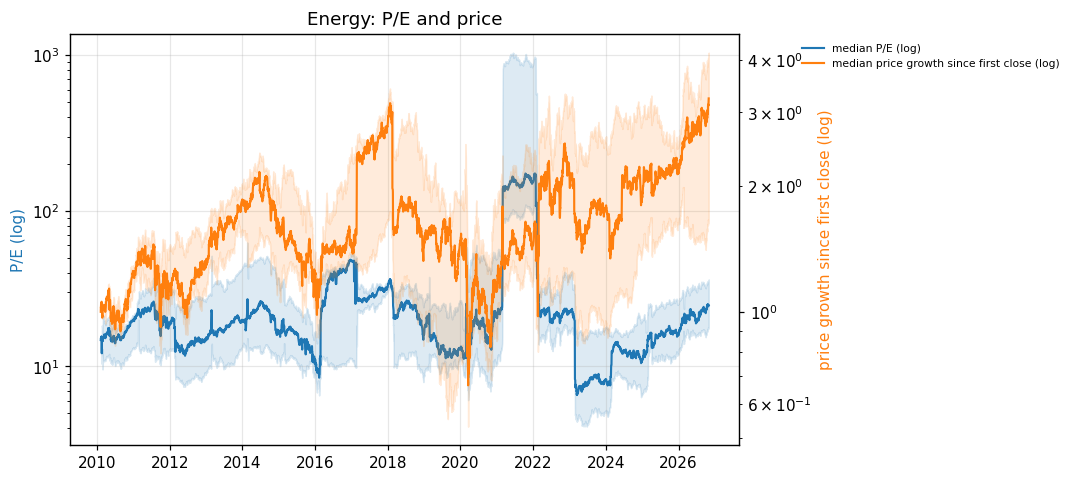
\includegraphics[width=\textwidth]{pe/sector_best.png}
\caption{Energy, the sector with the lowest median P/E (15.0): median P/E (left) and median price growth since each company's first close (right, log), each with its 25th to 75th percentile band.}
\end{figure}
\begin{figure}[H]
\centering
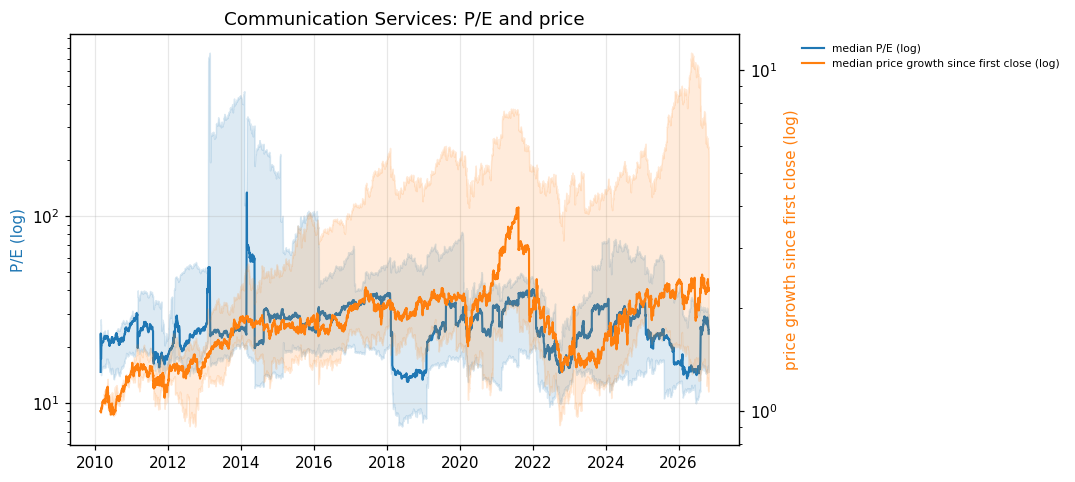
\includegraphics[width=\textwidth]{pe/sector_worst.png}
\caption{Communication Services, the sector with the highest median P/E (34.9): median P/E (left) and median price growth (right, log), with bands.}
\end{figure}
\subsection{Value against P/E: best and worst return}
The P/E of the sectors with the best and worst return against the S\&P 500, Information Technology and Communication Services.

\begin{figure}[H]
\centering
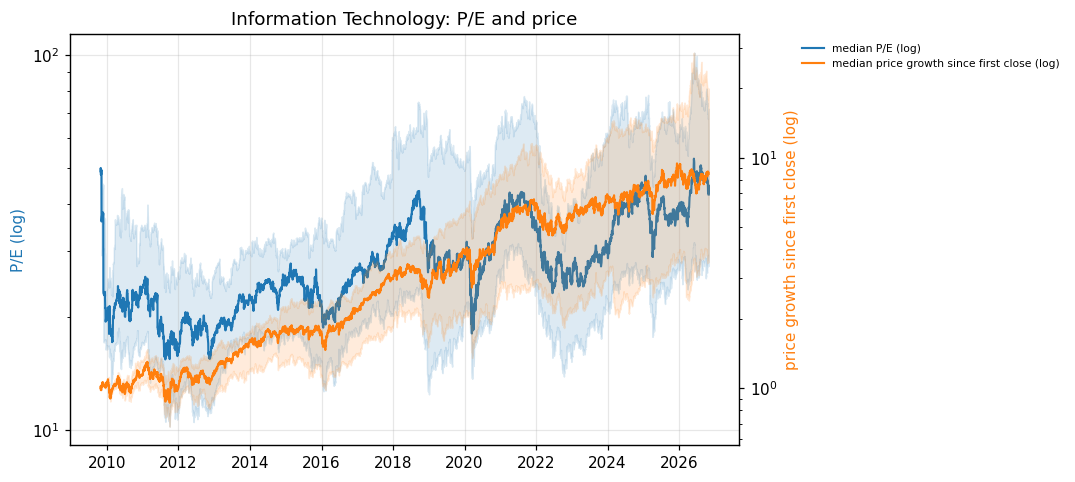
\includegraphics[width=\textwidth]{pe/value_best.png}
\caption{Information Technology, the sector with the best return against the S\&P 500: median P/E (left) and median price growth (right, log), with bands.}
\end{figure}
\begin{figure}[H]
\centering
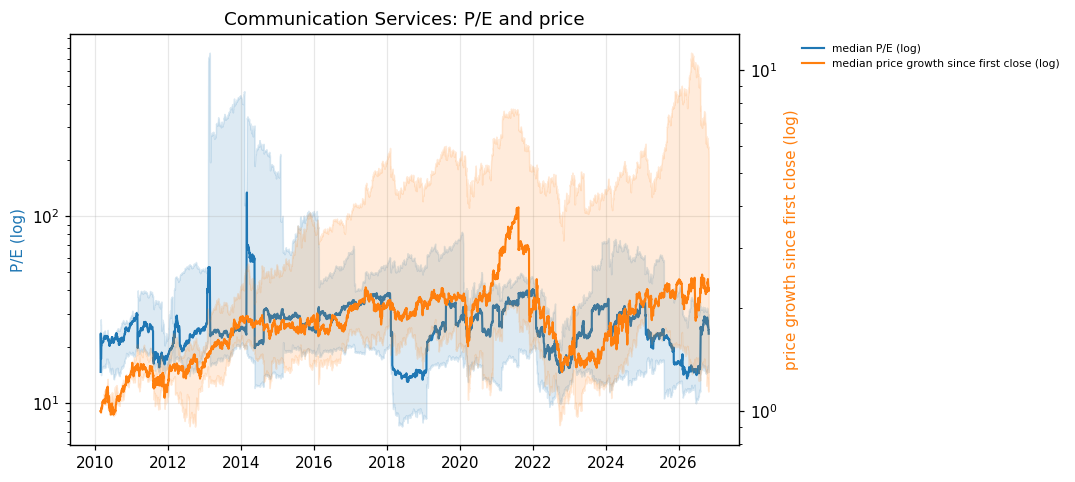
\includegraphics[width=\textwidth]{pe/value_worst.png}
\caption{Communication Services, the sector with the worst return against the S\&P 500: median P/E (left) and median price growth (right, log), with bands.}
\end{figure}
\subsection{Companies in Energy and Communication Services}
Within the sectors with the lowest and highest P/E, the five companies with the lowest P/E against the five with the highest.

\begin{figure}[H]
\centering
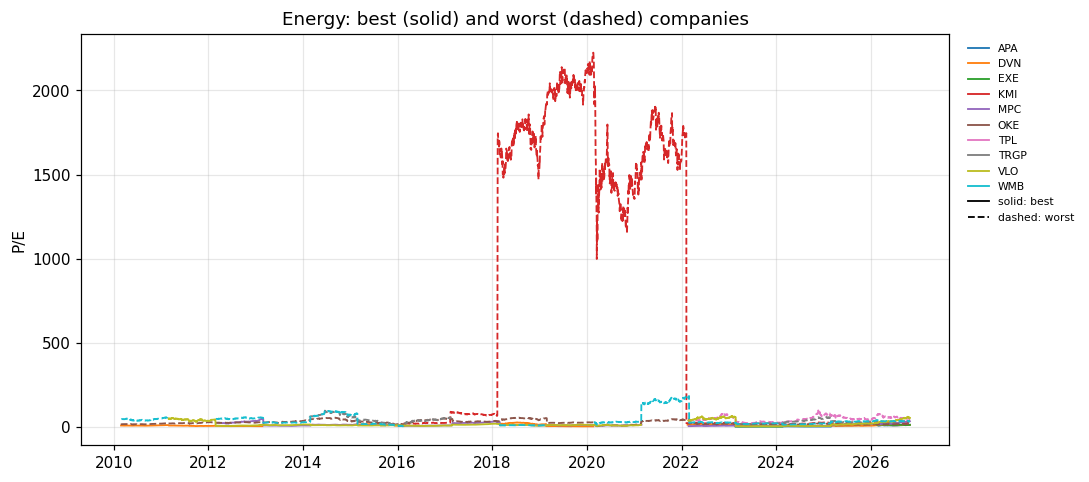
\includegraphics[width=\textwidth]{pe/companies_best.png}
\caption{Energy: P/E of the 5 companies with the lowest (solid) and highest (dashed) median P/E.}
\end{figure}
\begin{figure}[H]
\centering
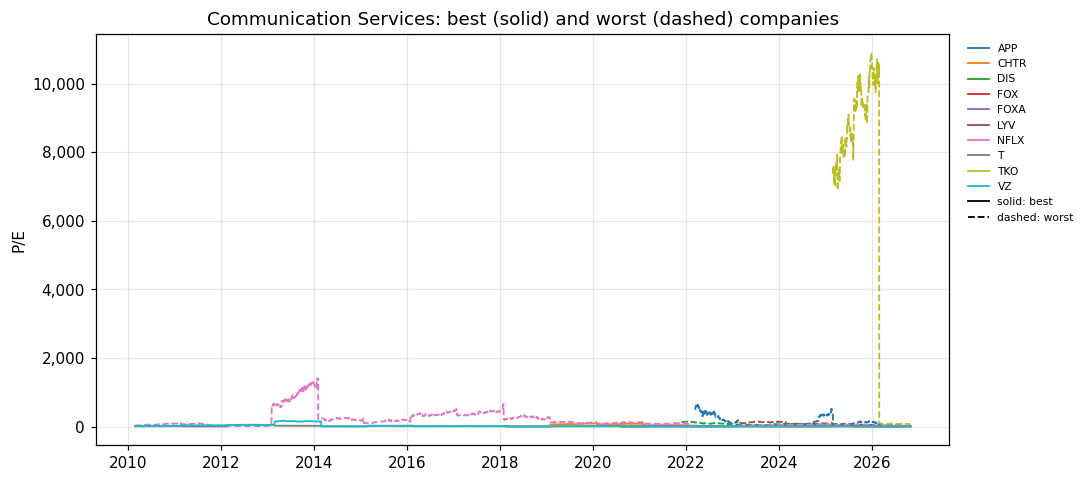
\includegraphics[width=\textwidth]{pe/companies_worst.png}
\caption{Communication Services: P/E of the 5 companies with the lowest (solid) and highest (dashed) median P/E.}
\end{figure}
\section{Dividend yield}
\label{sec:dividend_yield}
The trailing dividend yield is the sum of a company's dividends with an ex-date in the past twelve months divided by its share price, with both on the same split basis, in percent; a company that paid no dividend in the window yields zero. A company's score is its mean yield over the data; a sector's score is the median of its companies', and the highest is best.

\begin{figure}[H]
\centering
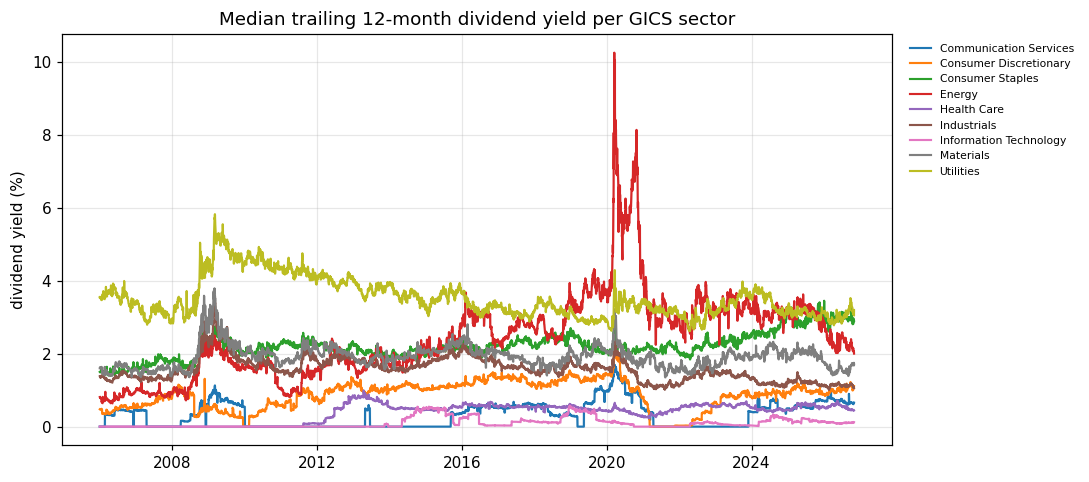
\includegraphics[width=\textwidth]{dividend_yield/summary.png}
\caption{Median trailing 12-month dividend yield of the companies in each GICS sector, percent.}
\end{figure}
\subsection{Best and worst sector}
Utilities pays the highest median yield (3.60\%) and Information Technology the lowest (0.35\%). Every sector's companies are in Appendix \ref{app:dividend_yield}.

\begin{figure}[H]
\centering
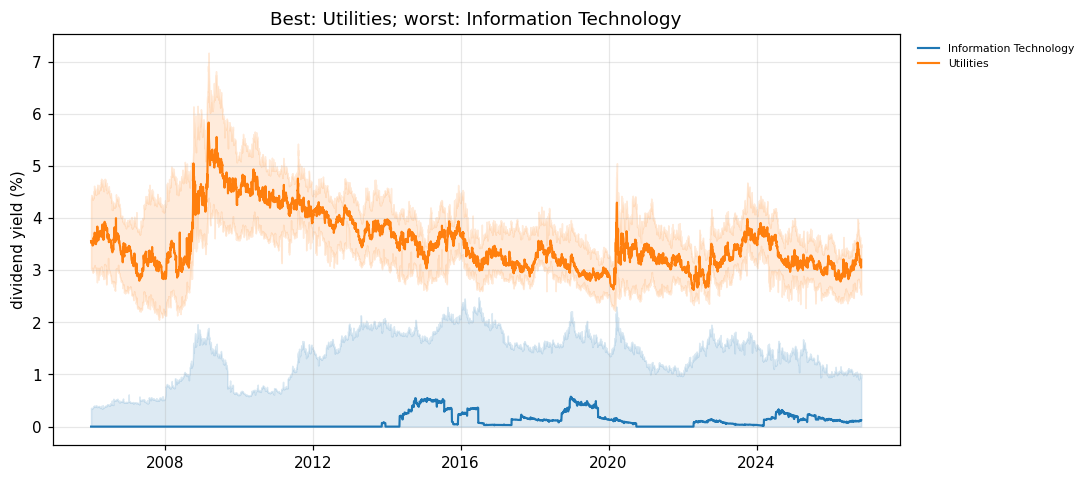
\includegraphics[width=\textwidth]{dividend_yield/sectors.png}
\caption{Median trailing dividend yield of Utilities (highest, 3.60\%) and Information Technology (lowest, 0.35\%), with their 25th to 75th percentile bands; percent.}
\end{figure}
\subsection{Companies in Utilities and Information Technology}
Within each of the two sectors, the five companies with the highest mean yield against the five with the lowest.

\begin{figure}[H]
\centering
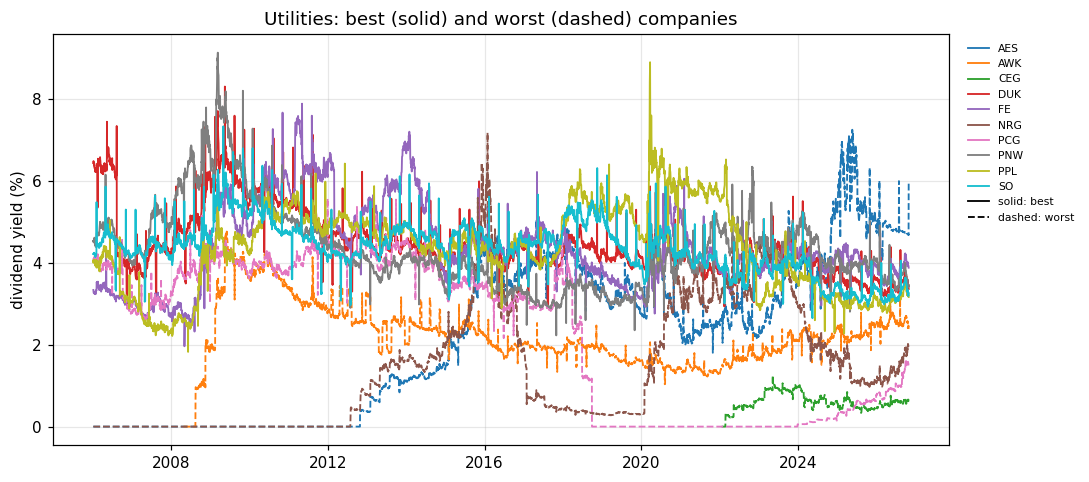
\includegraphics[width=\textwidth]{dividend_yield/companies_best.png}
\caption{Utilities: trailing dividend yield of the 5 companies with the highest (solid) and lowest (dashed) mean yield, percent.}
\end{figure}
\begin{figure}[H]
\centering
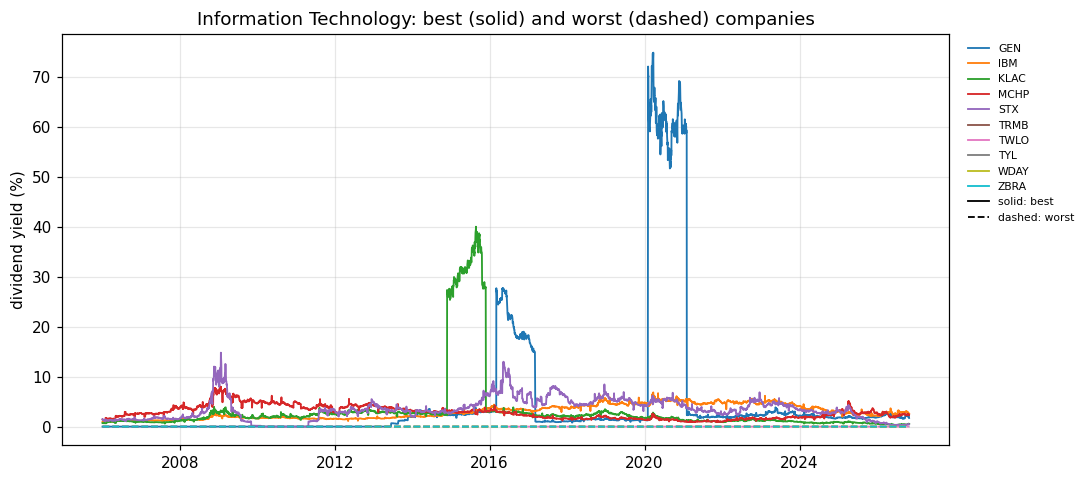
\includegraphics[width=\textwidth]{dividend_yield/companies_worst.png}
\caption{Information Technology: trailing dividend yield of the 5 companies with the highest (solid) and lowest (dashed) mean yield, percent.}
\end{figure}
\section{Data checks}
\label{sec:data_checks}
Checks of the data behind the sections above: how many companies report each field per year, whether reported EPS agrees with net income divided by diluted shares, how long after the period end filings arrive (the point-in-time delay), whether every symbol has a full trading calendar (youngest first, which shows each company's age in the data), and the exchange rate used for ZAR figures.

\begin{figure}[H]
\centering
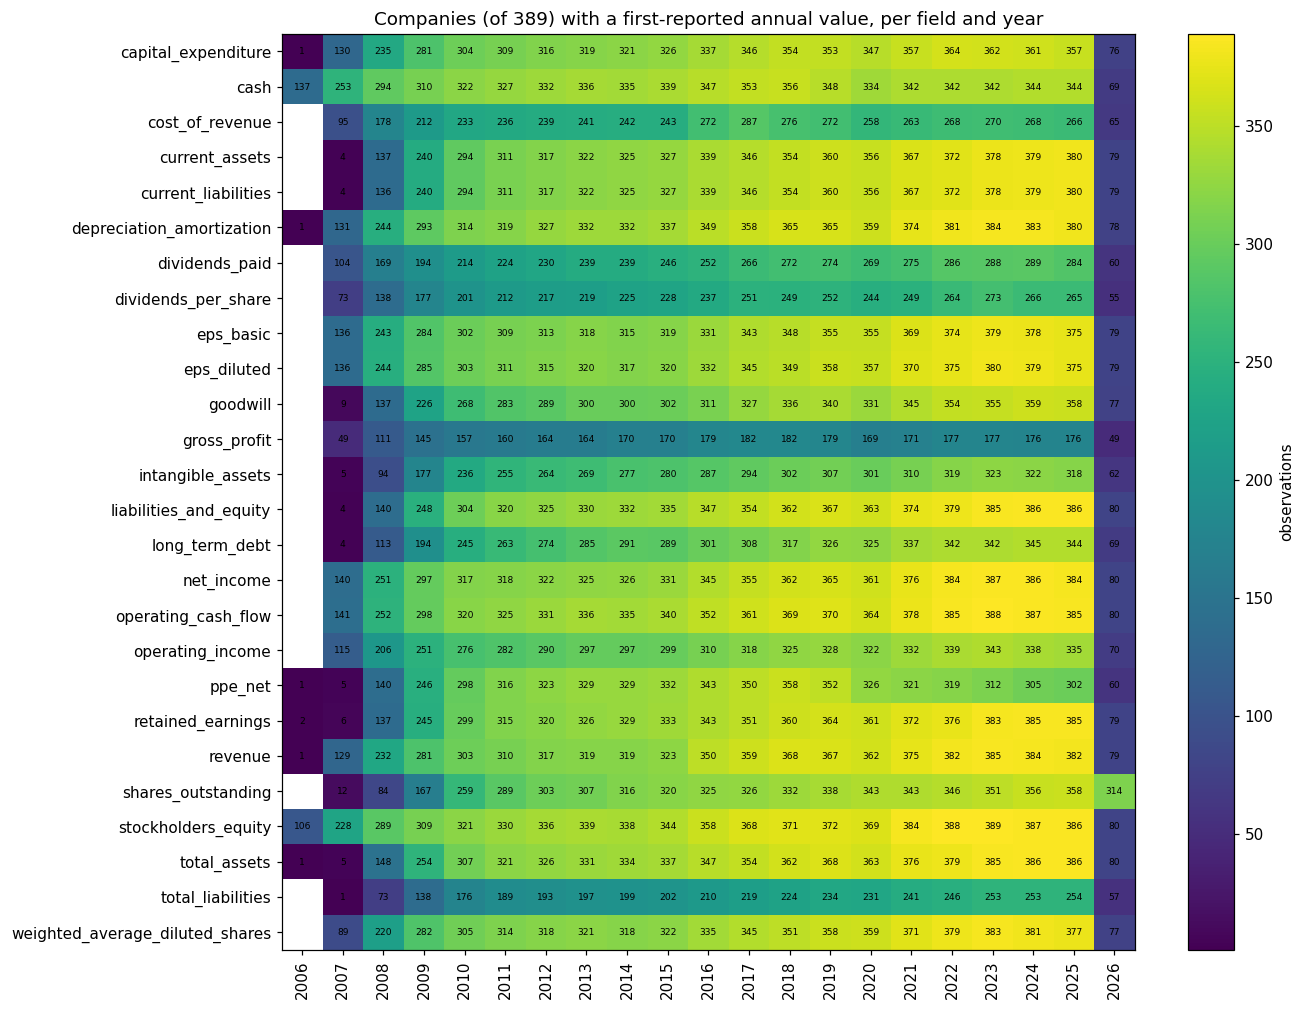
\includegraphics[width=\textwidth]{data_checks/coverage.png}
\caption{Number of companies with a first-reported annual value, per field and fiscal year.}
\end{figure}
\begin{figure}[H]
\centering
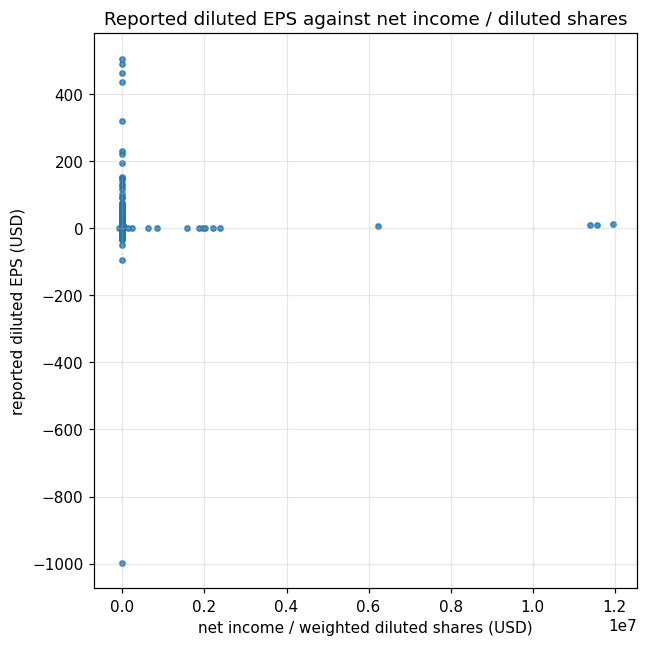
\includegraphics[width=\textwidth]{data_checks/eps_check.png}
\caption{Reported diluted EPS against net income divided by weighted diluted shares, USD per share; points off the diagonal differ.}
\end{figure}
\begin{figure}[H]
\centering
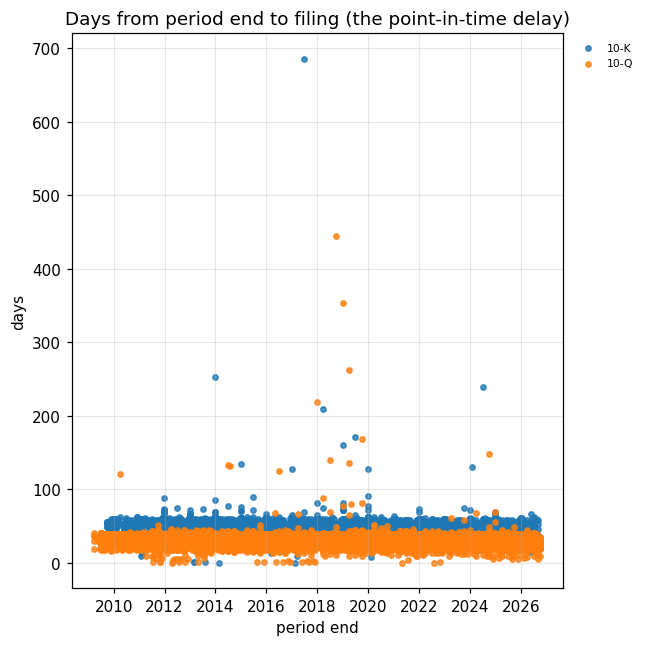
\includegraphics[width=\textwidth]{data_checks/filing_lag.png}
\caption{Days from period end to filing for each 10-K and 10-Q.}
\end{figure}
\begin{figure}[H]
\centering
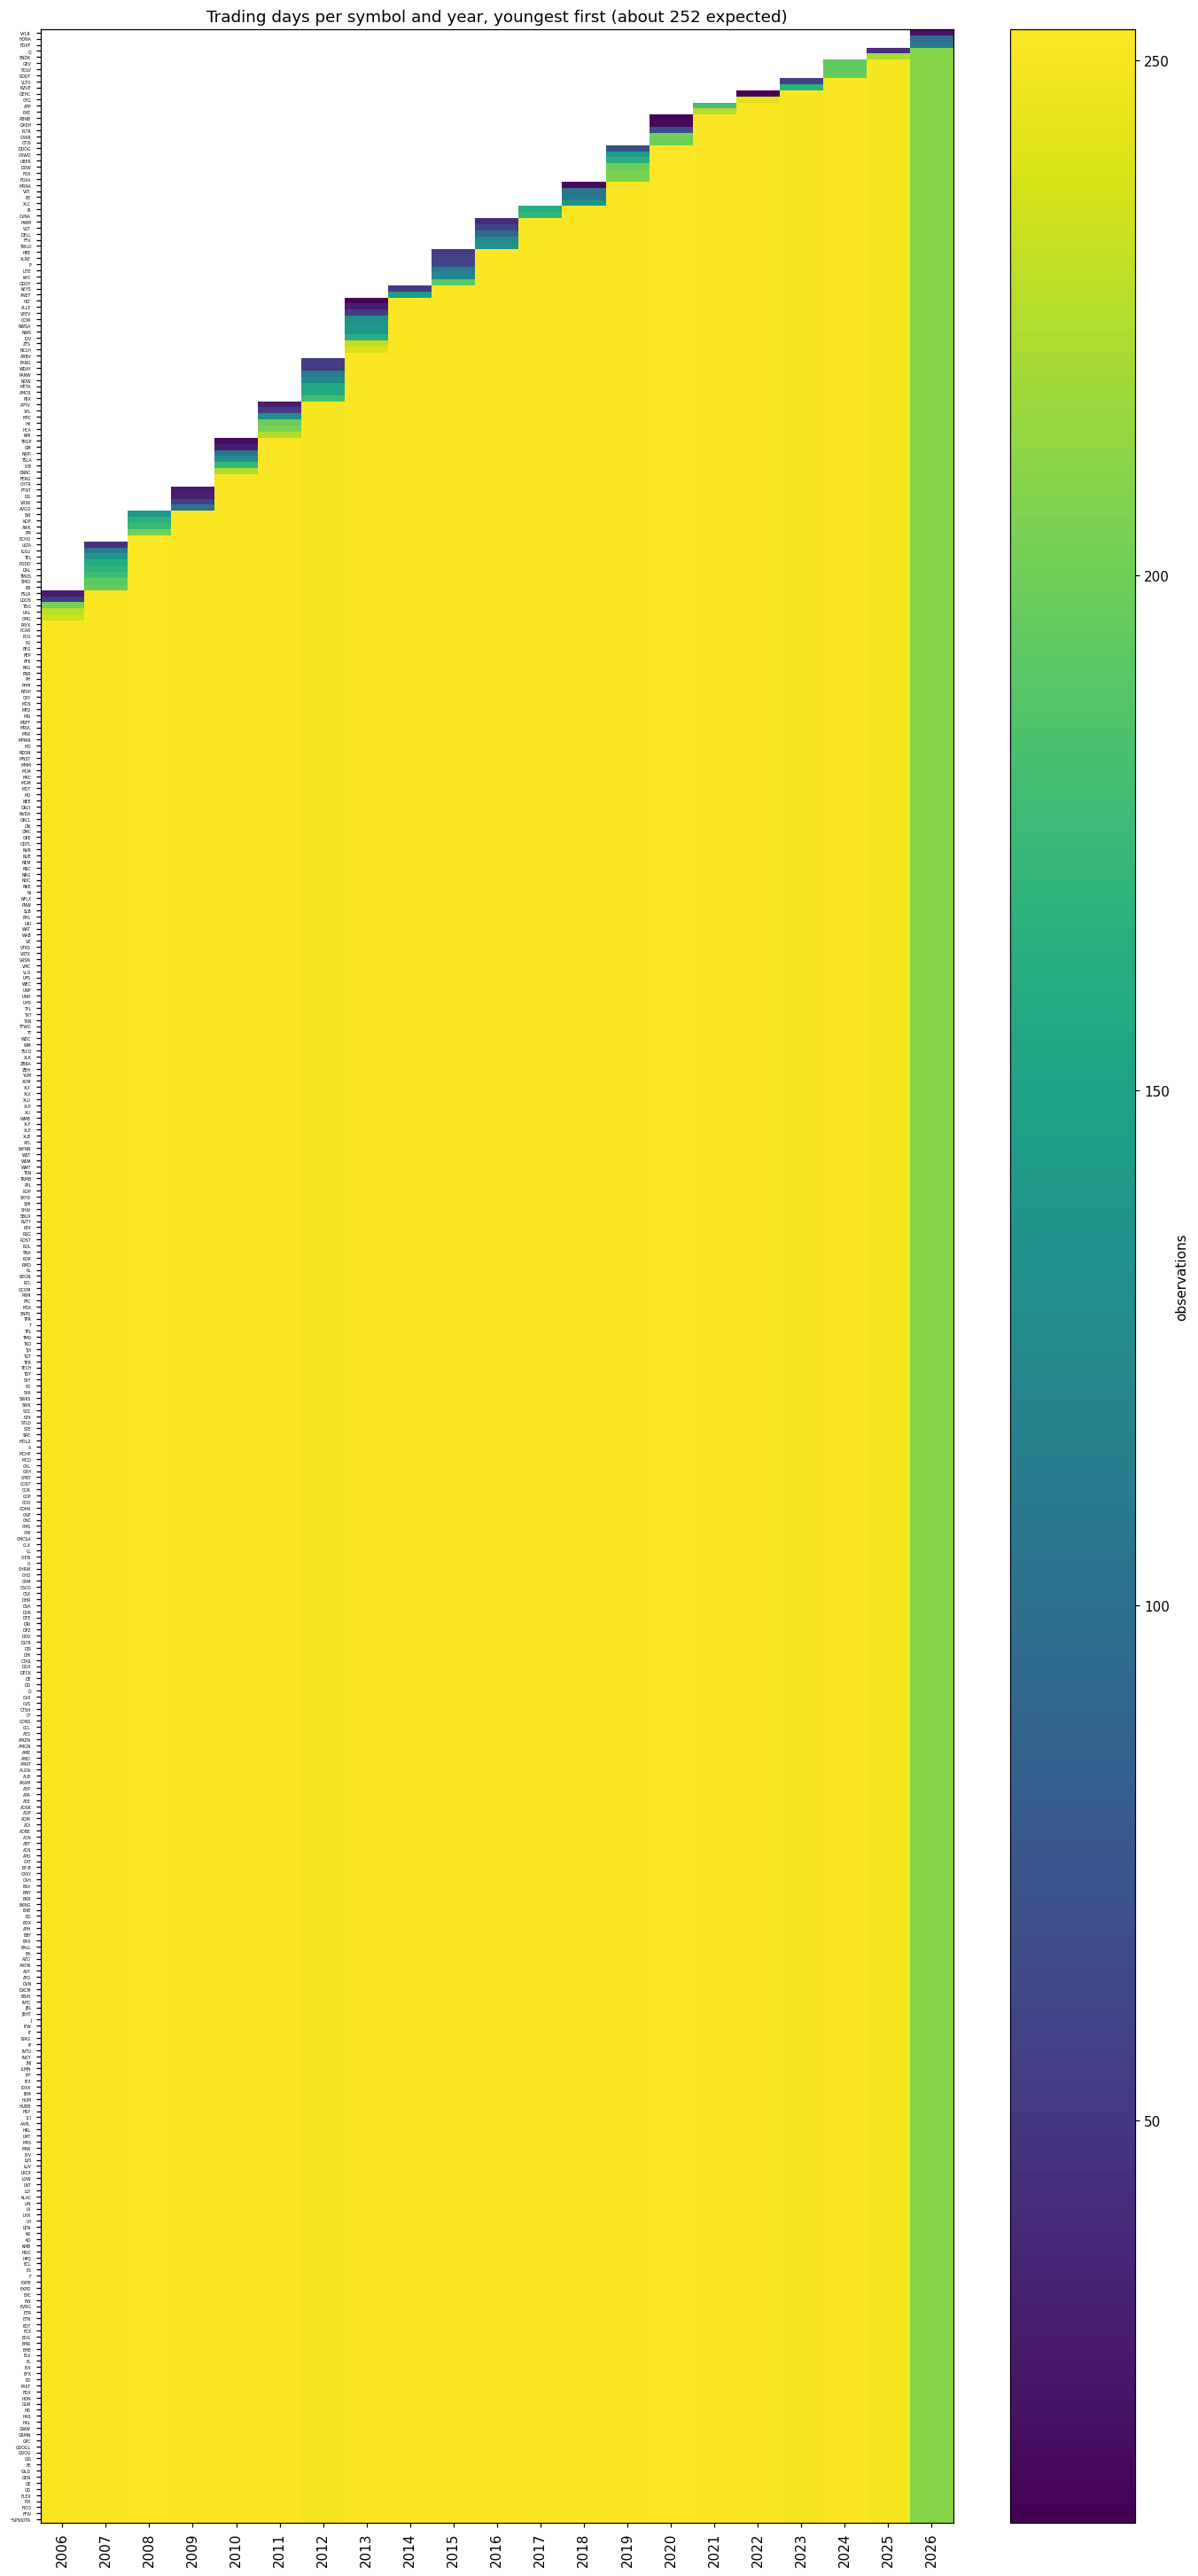
\includegraphics[width=\textwidth]{data_checks/trading_days.png}
\caption{Trading days per symbol and year, youngest symbols at the top; a row starts in the year the symbol first traded.}
\end{figure}
\begin{figure}[H]
\centering
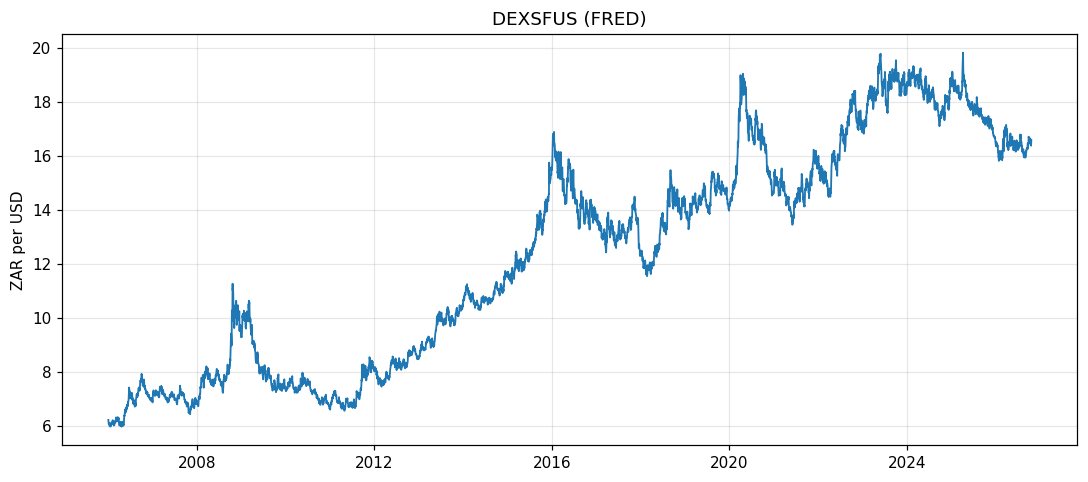
\includegraphics[width=\textwidth]{data_checks/DEXSFUS.png}
\caption{USD/ZAR exchange rate (FRED DEXSFUS), rand per US dollar.}
\end{figure}
\begin{figure}[H]
\centering
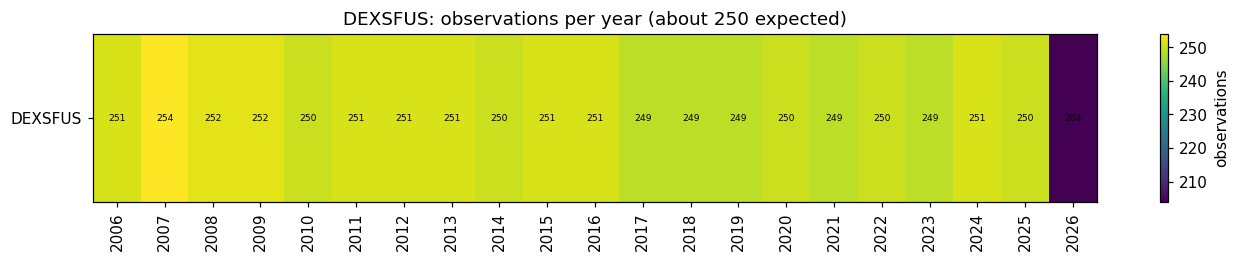
\includegraphics[width=\textwidth]{data_checks/DEXSFUS_coverage.png}
\caption{Exchange-rate observations per year.}
\end{figure}
\newpage
\appendix
\section{Fundamentals: revenue and net income: all GICS sectors}
\label{app:fundamentals}
For every GICS sector, its best companies (solid) against its worst (dashed) by the measure of the analysis.

\subsection{Communication Services}
\begin{figure}[H]
\centering
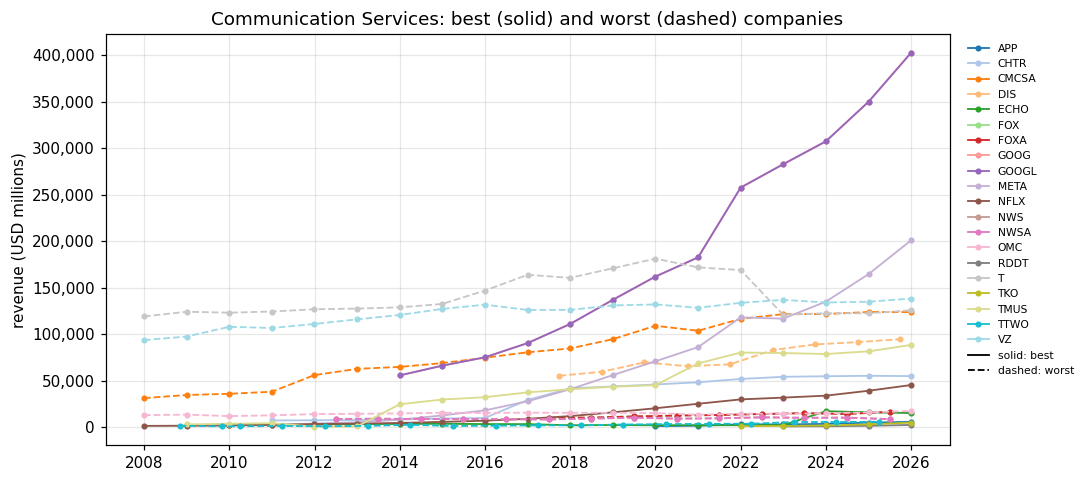
\includegraphics[width=\textwidth]{appendix/fundamentals/communication_services.png}
\caption{Communication Services: the 10 best (solid) and worst (dashed) companies by the measure of this analysis; fund XLC.}
\end{figure}
\subsection{Consumer Discretionary}
\begin{figure}[H]
\centering
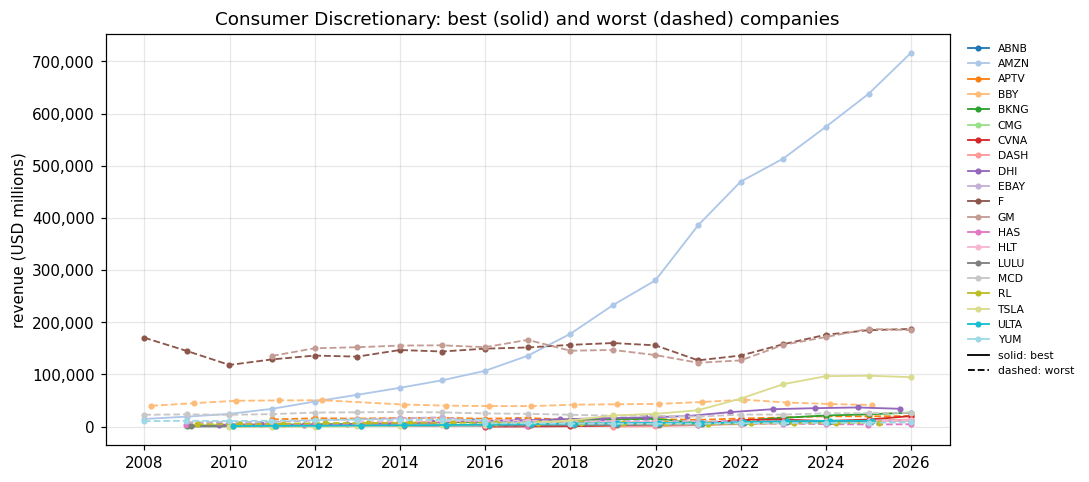
\includegraphics[width=\textwidth]{appendix/fundamentals/consumer_discretionary.png}
\caption{Consumer Discretionary: the 10 best (solid) and worst (dashed) companies by the measure of this analysis; fund XLY.}
\end{figure}
\subsection{Consumer Staples}
\begin{figure}[H]
\centering
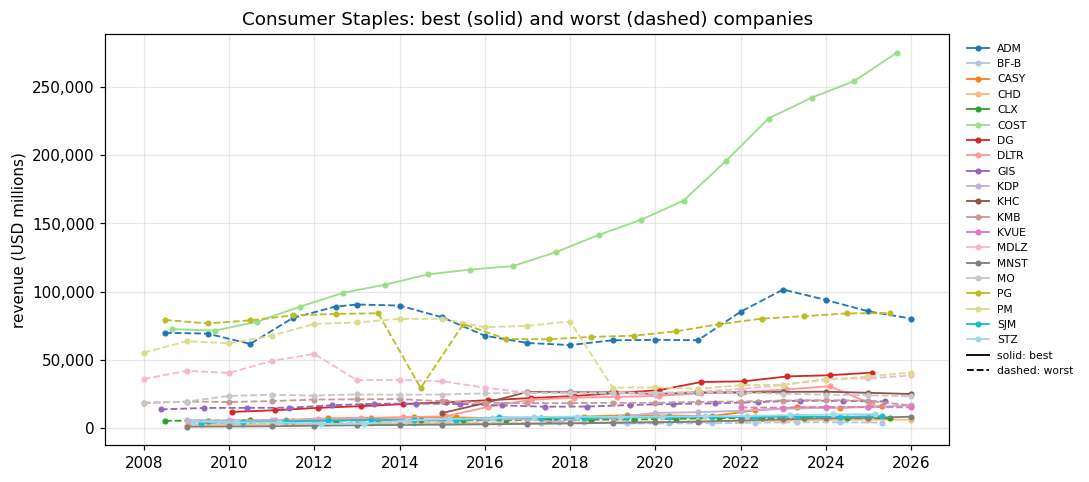
\includegraphics[width=\textwidth]{appendix/fundamentals/consumer_staples.png}
\caption{Consumer Staples: the 10 best (solid) and worst (dashed) companies by the measure of this analysis; fund XLP.}
\end{figure}
\subsection{Energy}
\begin{figure}[H]
\centering
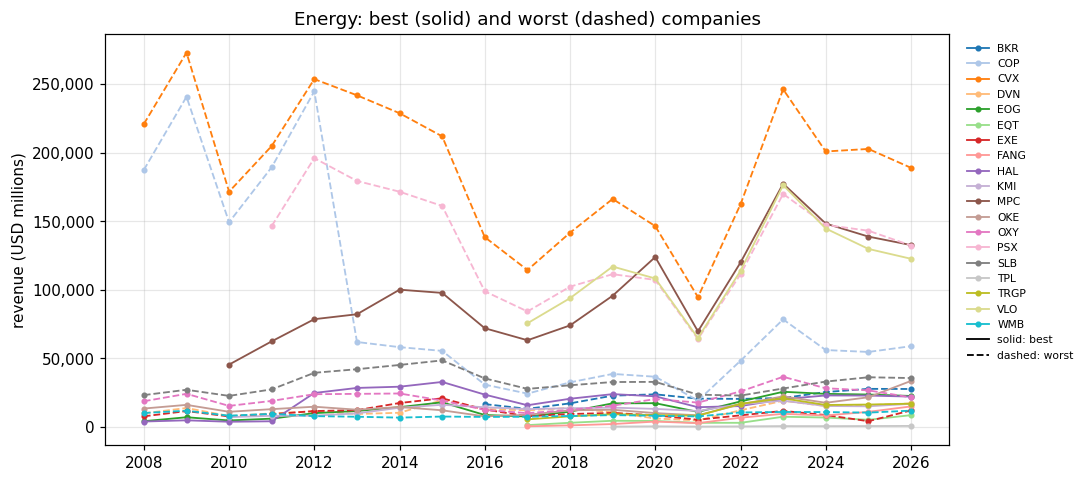
\includegraphics[width=\textwidth]{appendix/fundamentals/energy.png}
\caption{Energy: the 10 best (solid) and worst (dashed) companies by the measure of this analysis; fund XLE.}
\end{figure}
\subsection{Health Care}
\begin{figure}[H]
\centering
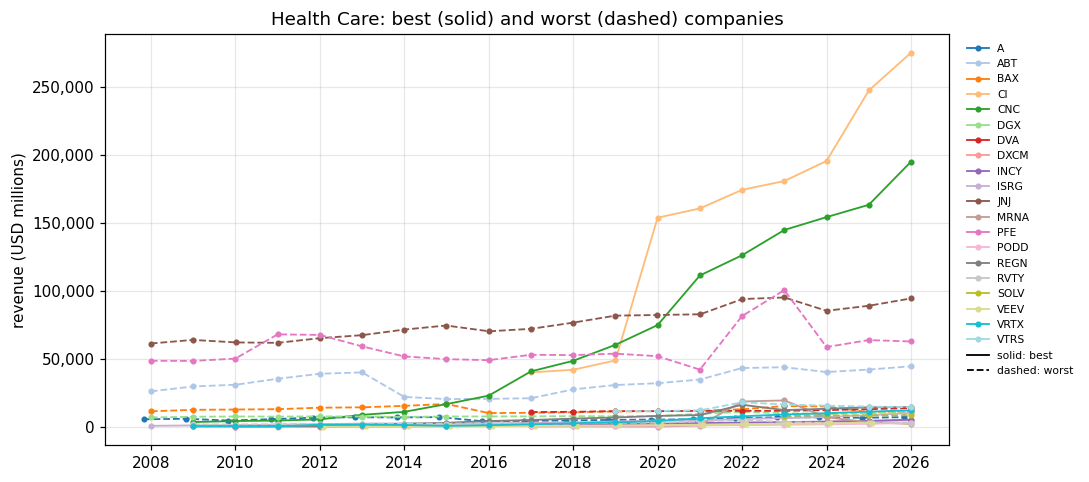
\includegraphics[width=\textwidth]{appendix/fundamentals/health_care.png}
\caption{Health Care: the 10 best (solid) and worst (dashed) companies by the measure of this analysis; fund XLV.}
\end{figure}
\subsection{Industrials}
\begin{figure}[H]
\centering
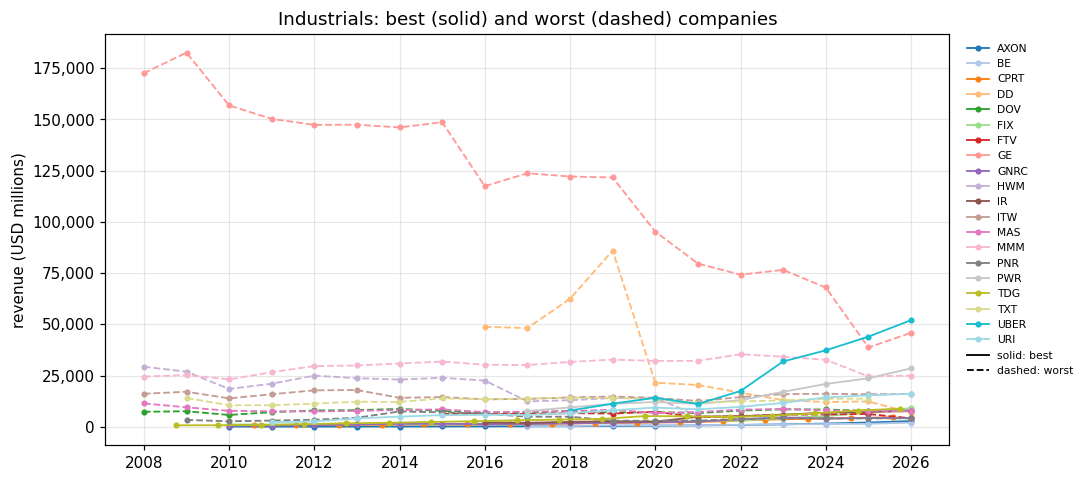
\includegraphics[width=\textwidth]{appendix/fundamentals/industrials.png}
\caption{Industrials: the 10 best (solid) and worst (dashed) companies by the measure of this analysis; fund XLI.}
\end{figure}
\subsection{Information Technology}
\begin{figure}[H]
\centering
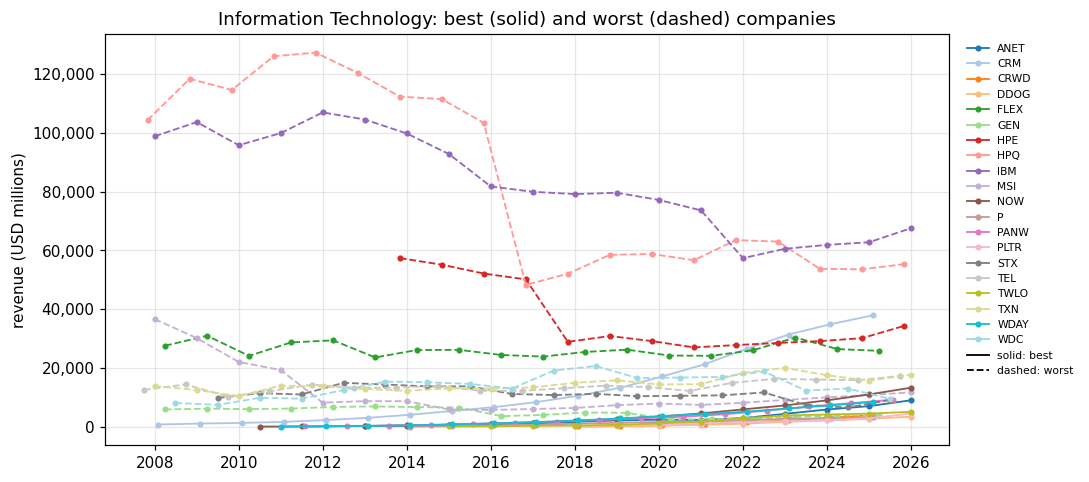
\includegraphics[width=\textwidth]{appendix/fundamentals/information_technology.png}
\caption{Information Technology: the 10 best (solid) and worst (dashed) companies by the measure of this analysis; fund XLK.}
\end{figure}
\subsection{Materials}
\begin{figure}[H]
\centering
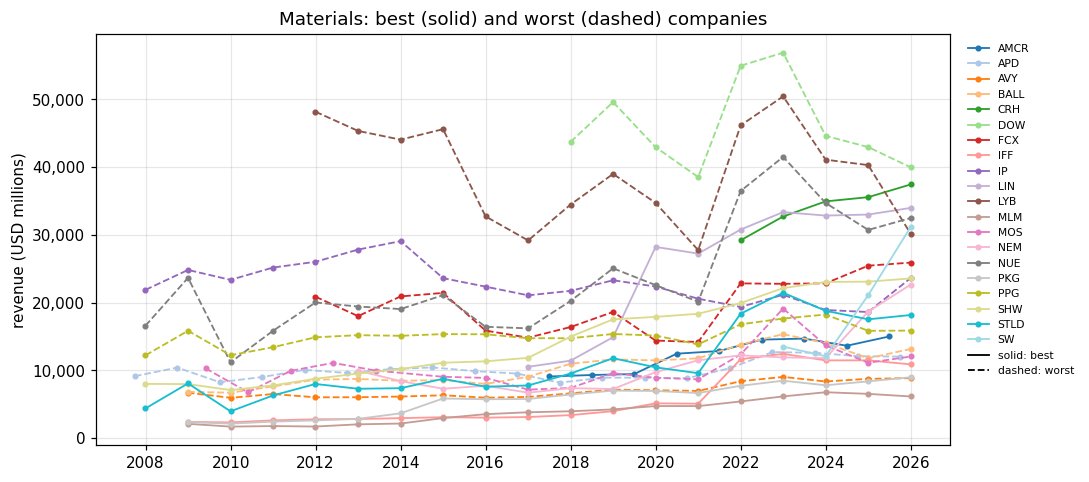
\includegraphics[width=\textwidth]{appendix/fundamentals/materials.png}
\caption{Materials: the 10 best (solid) and worst (dashed) companies by the measure of this analysis; fund XLB.}
\end{figure}
\subsection{Utilities}
\begin{figure}[H]
\centering
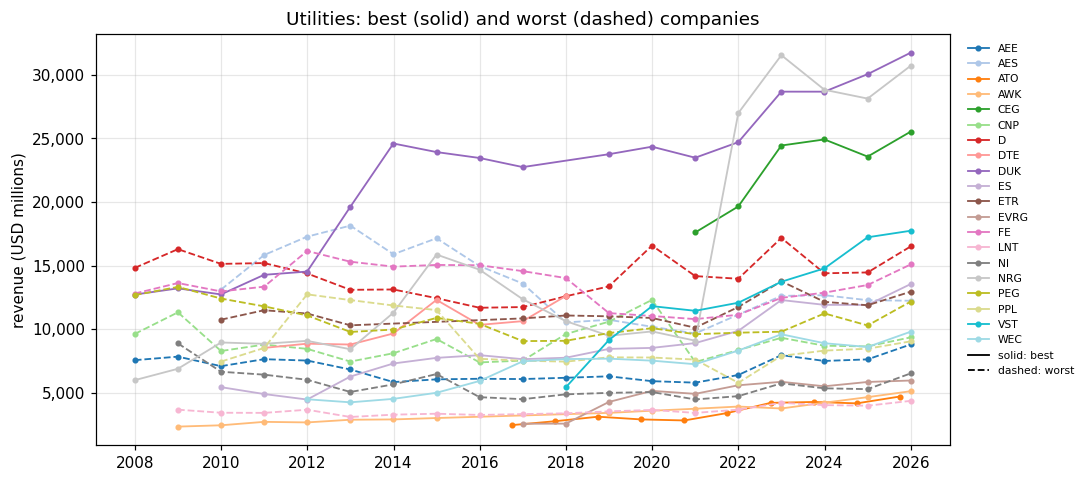
\includegraphics[width=\textwidth]{appendix/fundamentals/utilities.png}
\caption{Utilities: the 10 best (solid) and worst (dashed) companies by the measure of this analysis; fund XLU.}
\end{figure}
\section{Total return: all GICS sectors}
\label{app:total_return}
For every GICS sector, its best companies (solid) against its worst (dashed) by the measure of the analysis.

\subsection{Communication Services}
\begin{figure}[H]
\centering
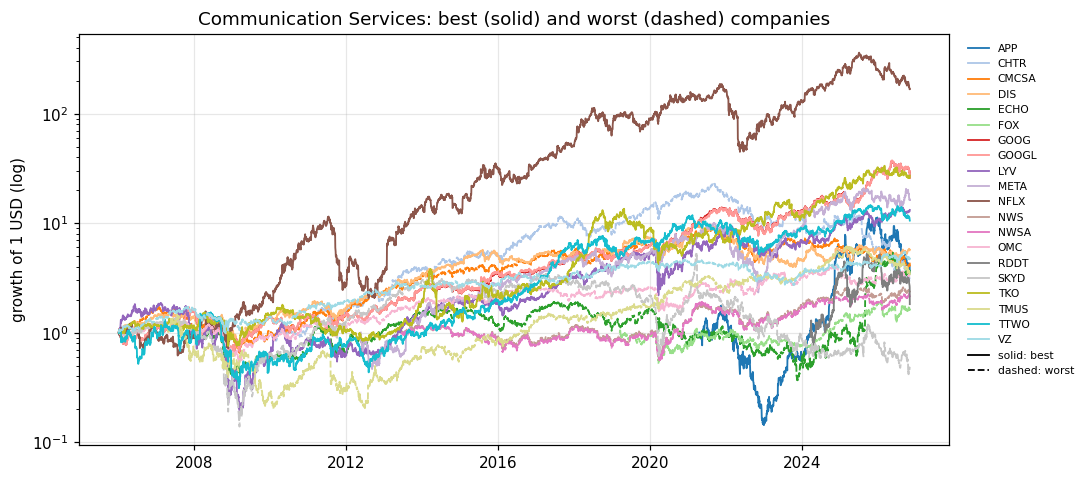
\includegraphics[width=\textwidth]{appendix/total_return/communication_services.png}
\caption{Communication Services: the 10 best (solid) and worst (dashed) companies by the measure of this analysis; fund XLC.}
\end{figure}
\subsection{Consumer Discretionary}
\begin{figure}[H]
\centering
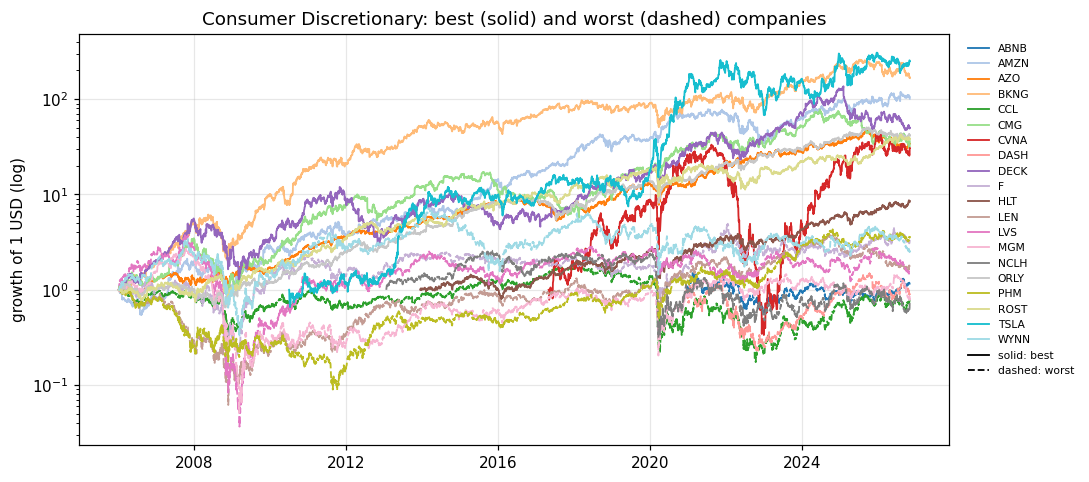
\includegraphics[width=\textwidth]{appendix/total_return/consumer_discretionary.png}
\caption{Consumer Discretionary: the 10 best (solid) and worst (dashed) companies by the measure of this analysis; fund XLY.}
\end{figure}
\subsection{Consumer Staples}
\begin{figure}[H]
\centering
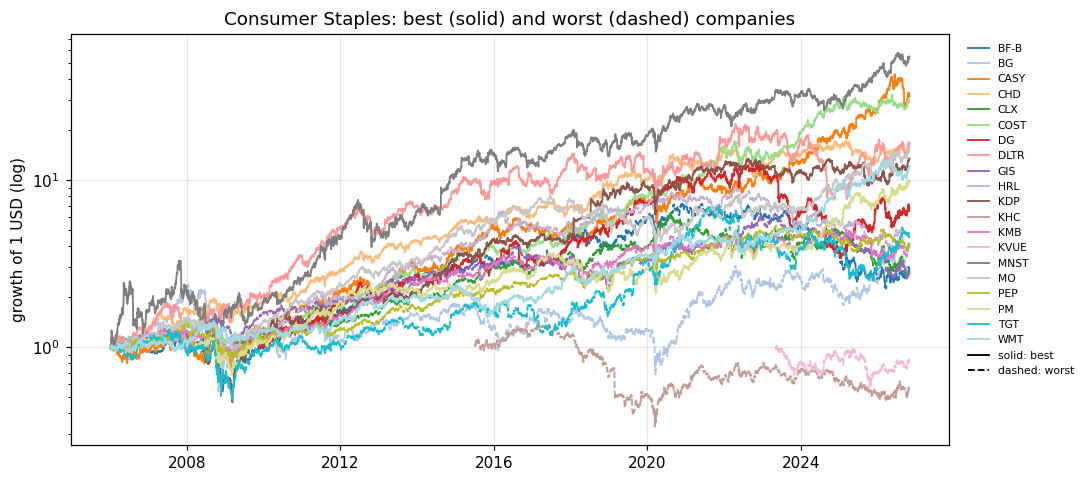
\includegraphics[width=\textwidth]{appendix/total_return/consumer_staples.png}
\caption{Consumer Staples: the 10 best (solid) and worst (dashed) companies by the measure of this analysis; fund XLP.}
\end{figure}
\subsection{Energy}
\begin{figure}[H]
\centering
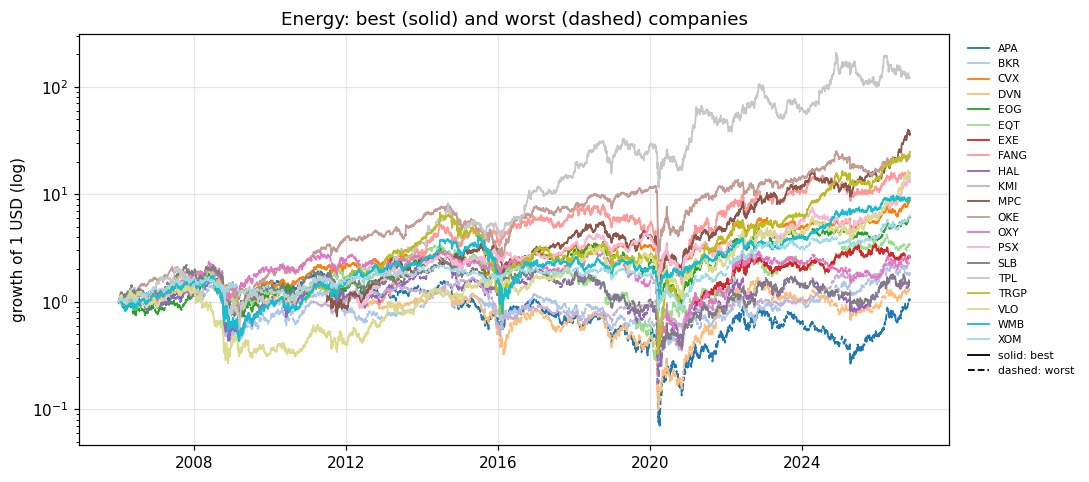
\includegraphics[width=\textwidth]{appendix/total_return/energy.png}
\caption{Energy: the 10 best (solid) and worst (dashed) companies by the measure of this analysis; fund XLE.}
\end{figure}
\subsection{Health Care}
\begin{figure}[H]
\centering
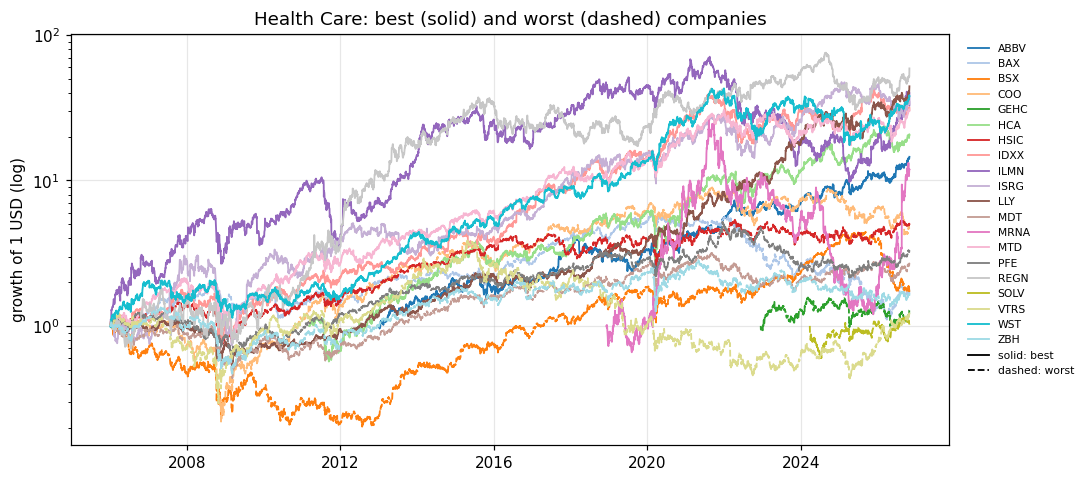
\includegraphics[width=\textwidth]{appendix/total_return/health_care.png}
\caption{Health Care: the 10 best (solid) and worst (dashed) companies by the measure of this analysis; fund XLV.}
\end{figure}
\subsection{Industrials}
\begin{figure}[H]
\centering
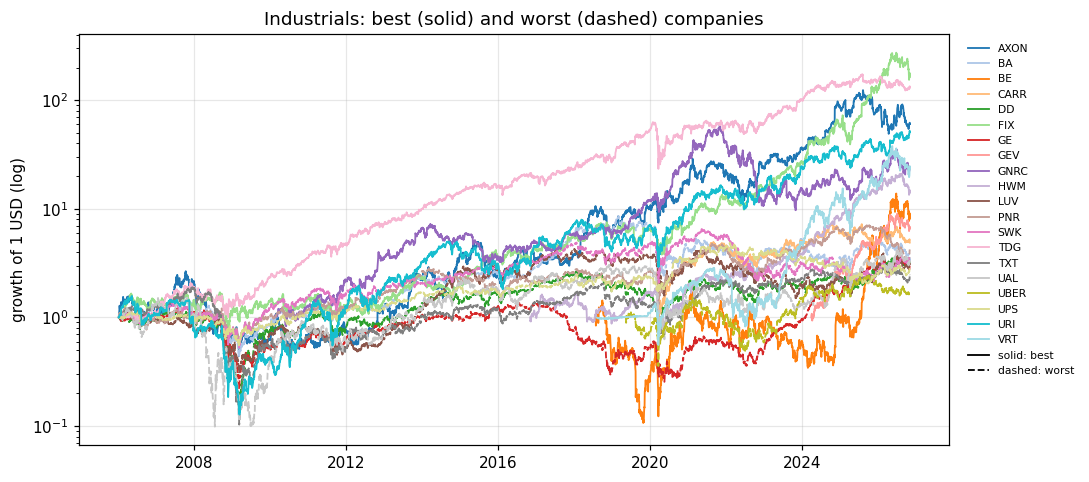
\includegraphics[width=\textwidth]{appendix/total_return/industrials.png}
\caption{Industrials: the 10 best (solid) and worst (dashed) companies by the measure of this analysis; fund XLI.}
\end{figure}
\subsection{Information Technology}
\begin{figure}[H]
\centering
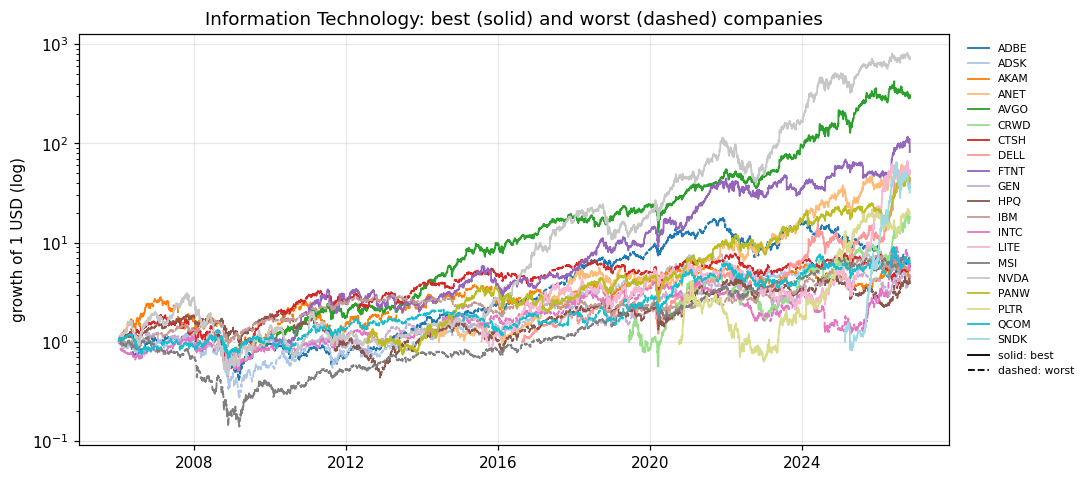
\includegraphics[width=\textwidth]{appendix/total_return/information_technology.png}
\caption{Information Technology: the 10 best (solid) and worst (dashed) companies by the measure of this analysis; fund XLK.}
\end{figure}
\subsection{Materials}
\begin{figure}[H]
\centering
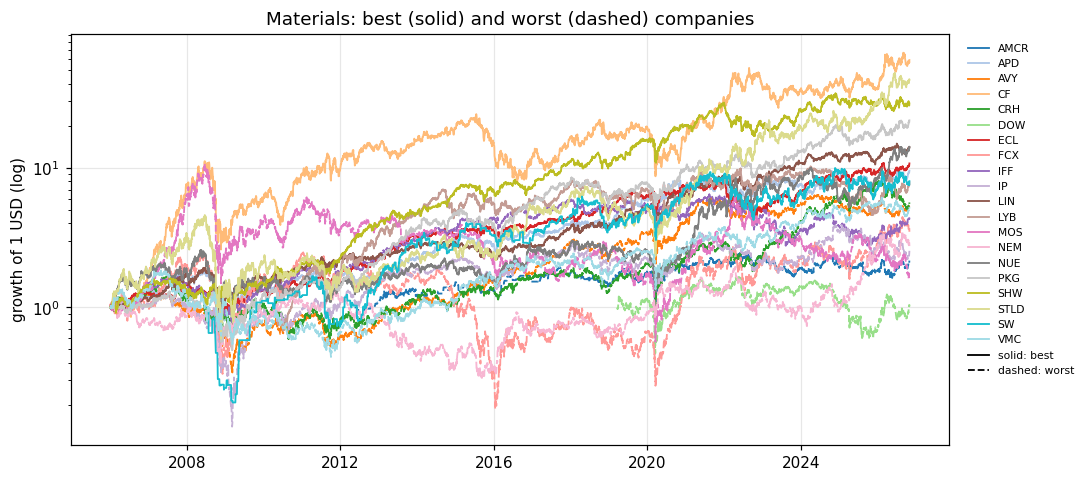
\includegraphics[width=\textwidth]{appendix/total_return/materials.png}
\caption{Materials: the 10 best (solid) and worst (dashed) companies by the measure of this analysis; fund XLB.}
\end{figure}
\subsection{Utilities}
\begin{figure}[H]
\centering
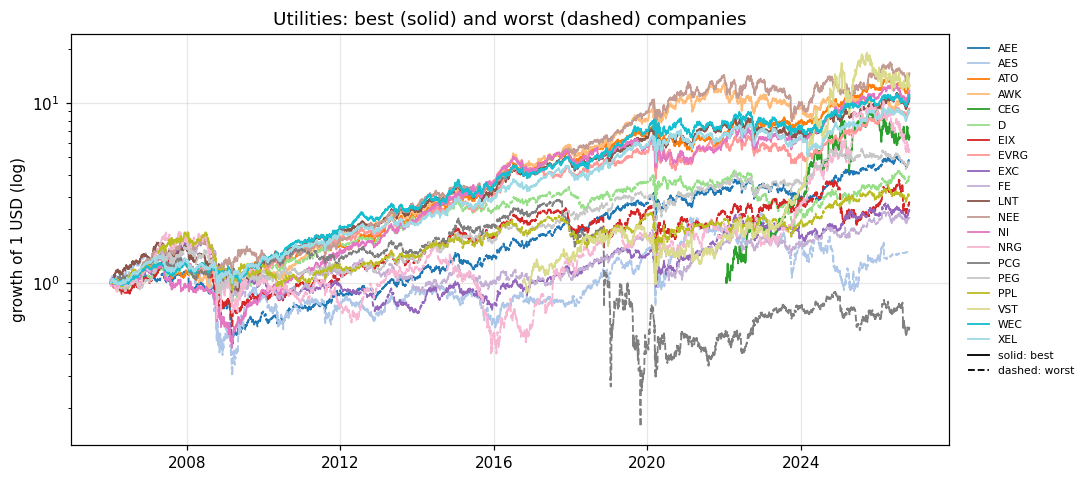
\includegraphics[width=\textwidth]{appendix/total_return/utilities.png}
\caption{Utilities: the 10 best (solid) and worst (dashed) companies by the measure of this analysis; fund XLU.}
\end{figure}
\section{Relative return: all GICS sectors}
\label{app:relative_return}
For every GICS sector, its best companies (solid) against its worst (dashed) by the measure of the analysis.

\subsection{Communication Services}
\begin{figure}[H]
\centering
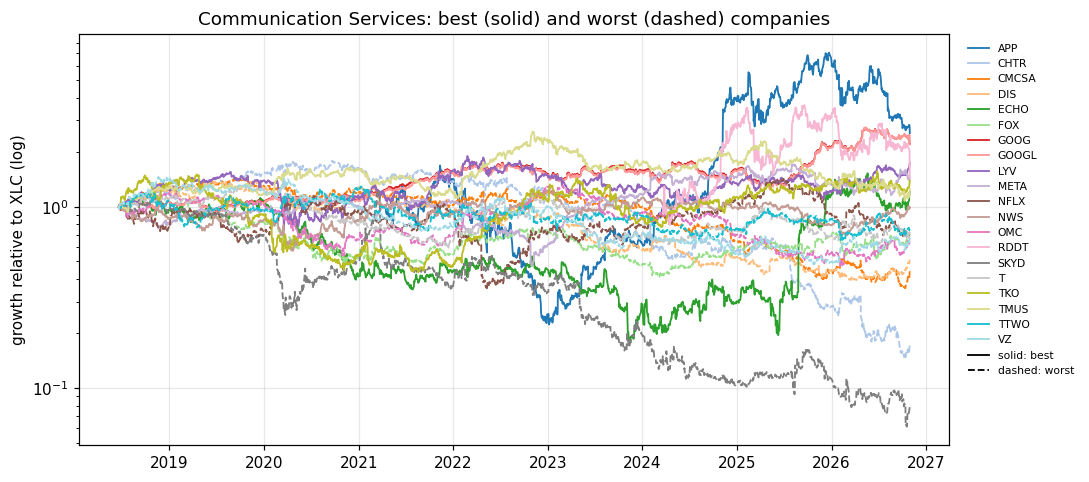
\includegraphics[width=\textwidth]{appendix/relative_return/communication_services.png}
\caption{Communication Services: the 10 best (solid) and worst (dashed) companies by the measure of this analysis; fund XLC.}
\end{figure}
\subsection{Consumer Discretionary}
\begin{figure}[H]
\centering
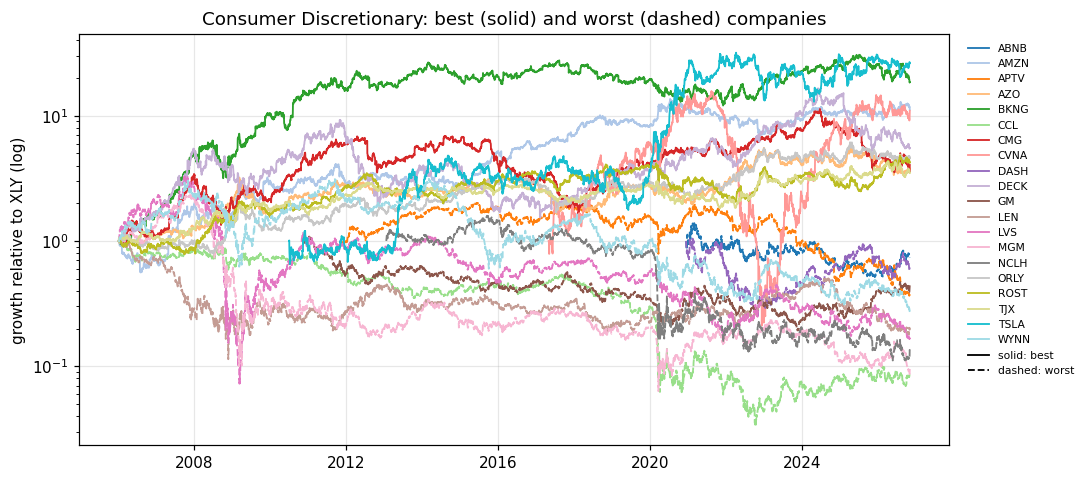
\includegraphics[width=\textwidth]{appendix/relative_return/consumer_discretionary.png}
\caption{Consumer Discretionary: the 10 best (solid) and worst (dashed) companies by the measure of this analysis; fund XLY.}
\end{figure}
\subsection{Consumer Staples}
\begin{figure}[H]
\centering
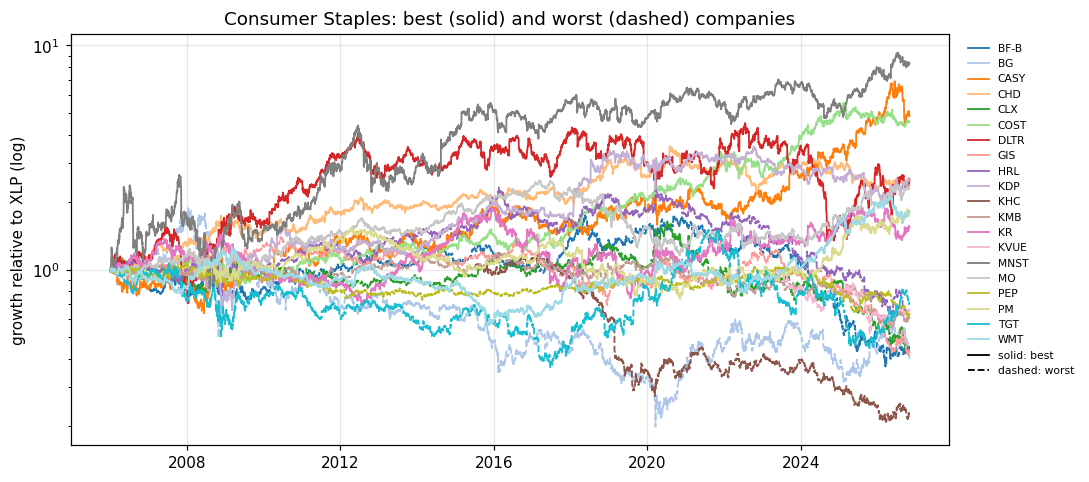
\includegraphics[width=\textwidth]{appendix/relative_return/consumer_staples.png}
\caption{Consumer Staples: the 10 best (solid) and worst (dashed) companies by the measure of this analysis; fund XLP.}
\end{figure}
\subsection{Energy}
\begin{figure}[H]
\centering
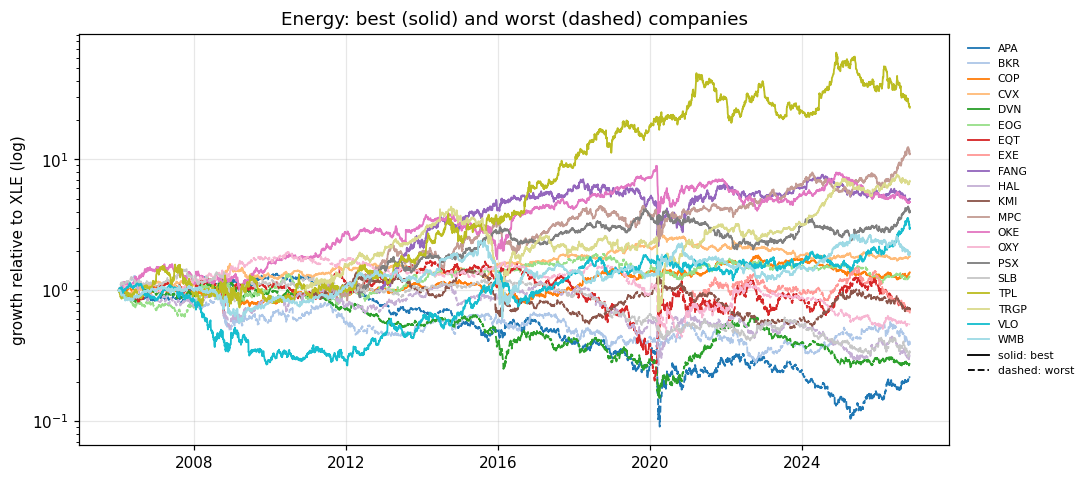
\includegraphics[width=\textwidth]{appendix/relative_return/energy.png}
\caption{Energy: the 10 best (solid) and worst (dashed) companies by the measure of this analysis; fund XLE.}
\end{figure}
\subsection{Health Care}
\begin{figure}[H]
\centering
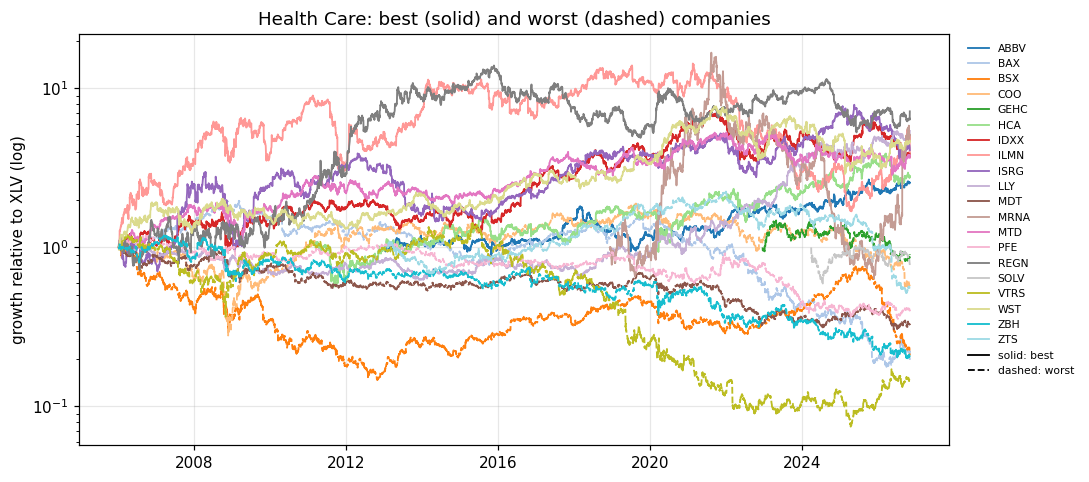
\includegraphics[width=\textwidth]{appendix/relative_return/health_care.png}
\caption{Health Care: the 10 best (solid) and worst (dashed) companies by the measure of this analysis; fund XLV.}
\end{figure}
\subsection{Industrials}
\begin{figure}[H]
\centering
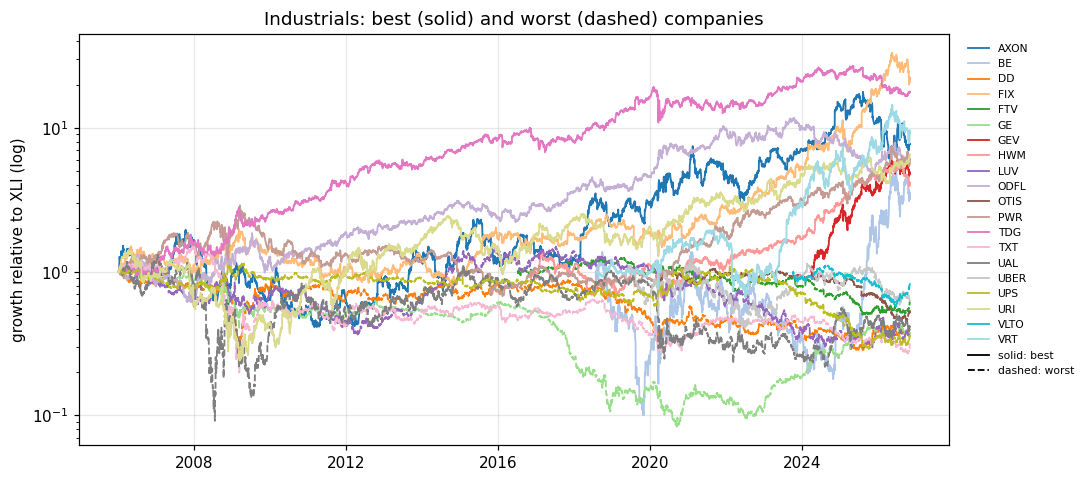
\includegraphics[width=\textwidth]{appendix/relative_return/industrials.png}
\caption{Industrials: the 10 best (solid) and worst (dashed) companies by the measure of this analysis; fund XLI.}
\end{figure}
\subsection{Information Technology}
\begin{figure}[H]
\centering
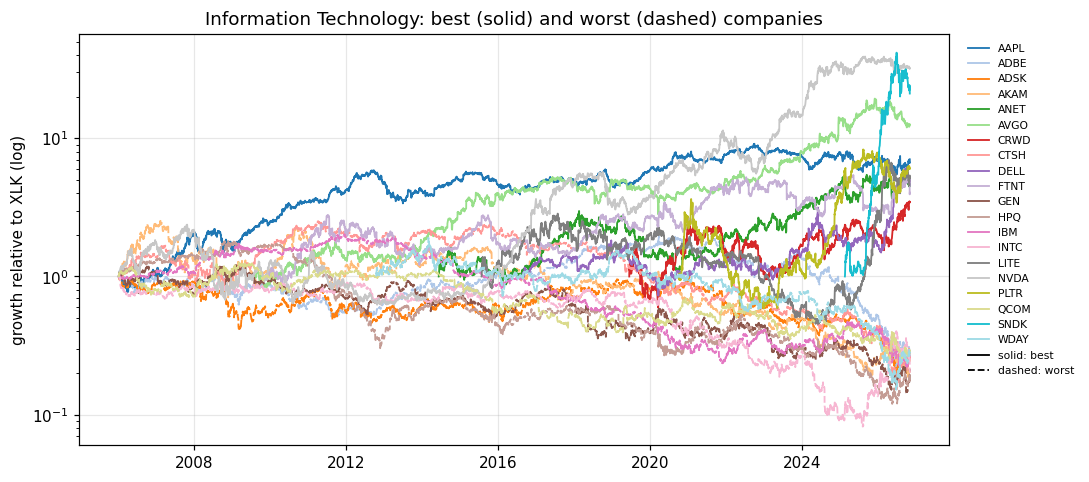
\includegraphics[width=\textwidth]{appendix/relative_return/information_technology.png}
\caption{Information Technology: the 10 best (solid) and worst (dashed) companies by the measure of this analysis; fund XLK.}
\end{figure}
\subsection{Materials}
\begin{figure}[H]
\centering
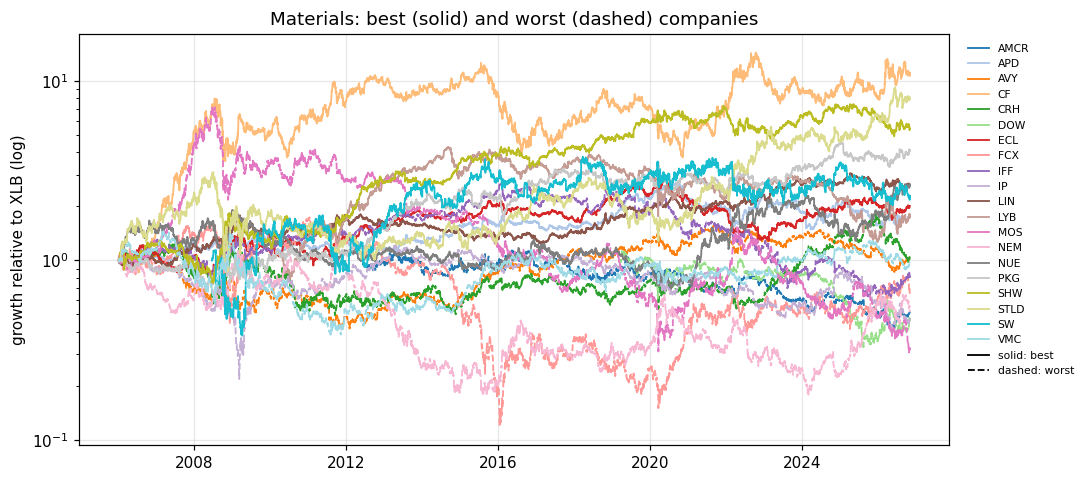
\includegraphics[width=\textwidth]{appendix/relative_return/materials.png}
\caption{Materials: the 10 best (solid) and worst (dashed) companies by the measure of this analysis; fund XLB.}
\end{figure}
\subsection{Utilities}
\begin{figure}[H]
\centering
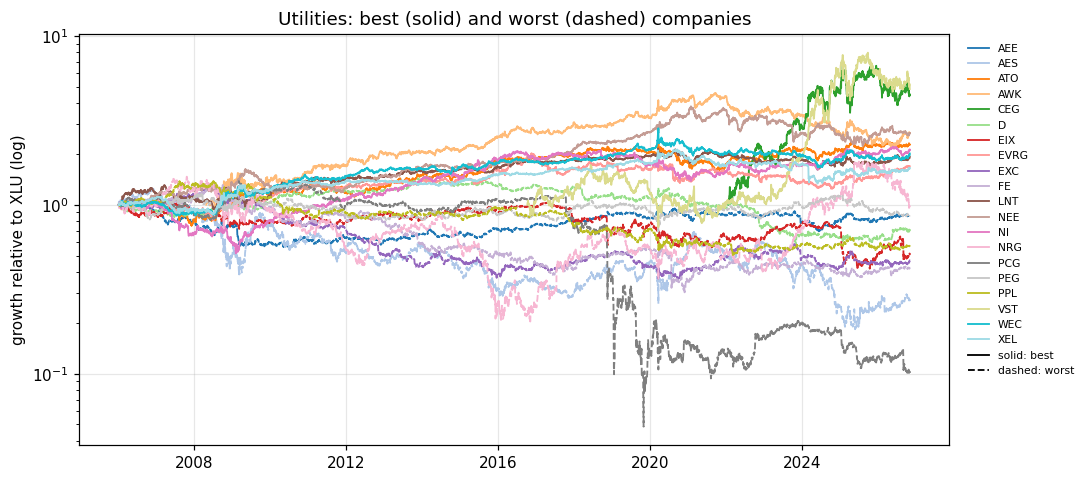
\includegraphics[width=\textwidth]{appendix/relative_return/utilities.png}
\caption{Utilities: the 10 best (solid) and worst (dashed) companies by the measure of this analysis; fund XLU.}
\end{figure}
\section{Price-to-earnings ratio: all GICS sectors}
\label{app:pe}
For every GICS sector, its best companies (solid) against its worst (dashed) by the measure of the analysis.

\subsection{Communication Services}
\begin{figure}[H]
\centering
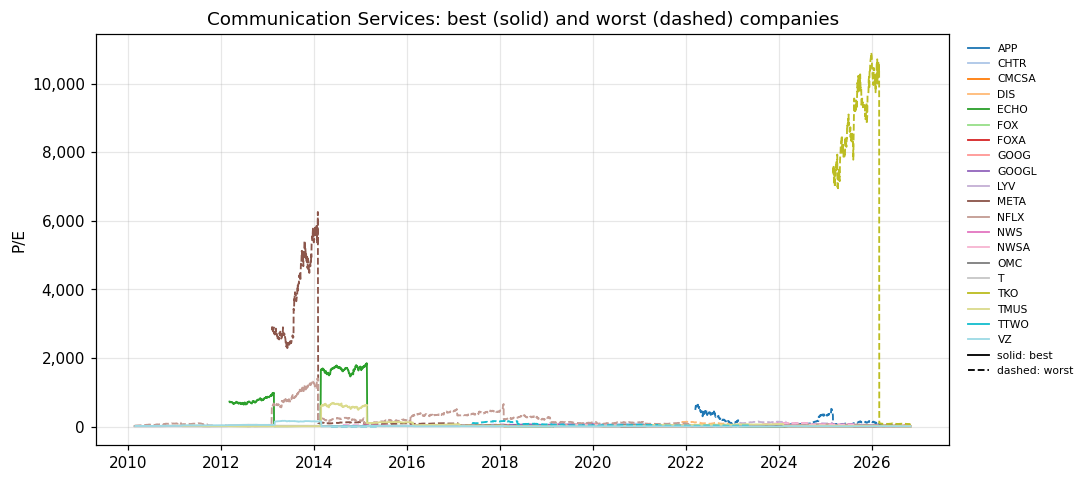
\includegraphics[width=\textwidth]{appendix/pe/communication_services.png}
\caption{Communication Services: the 10 best (solid) and worst (dashed) companies by the measure of this analysis; fund XLC.}
\end{figure}
\subsection{Consumer Discretionary}
\begin{figure}[H]
\centering
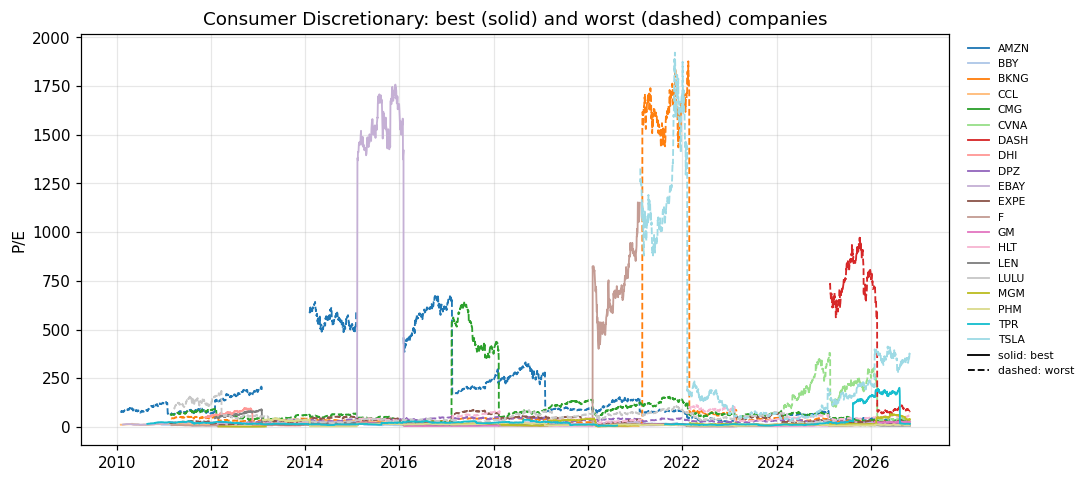
\includegraphics[width=\textwidth]{appendix/pe/consumer_discretionary.png}
\caption{Consumer Discretionary: the 10 best (solid) and worst (dashed) companies by the measure of this analysis; fund XLY.}
\end{figure}
\subsection{Consumer Staples}
\begin{figure}[H]
\centering
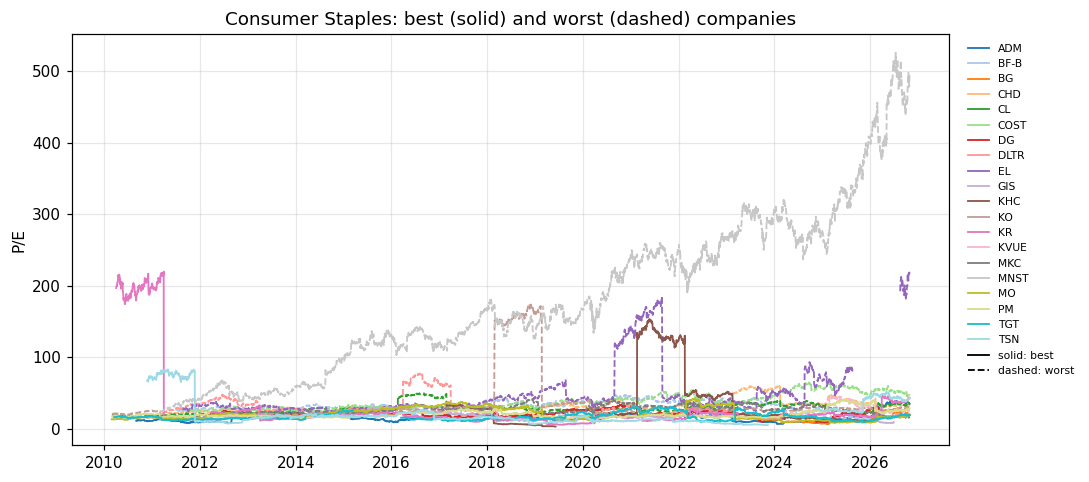
\includegraphics[width=\textwidth]{appendix/pe/consumer_staples.png}
\caption{Consumer Staples: the 10 best (solid) and worst (dashed) companies by the measure of this analysis; fund XLP.}
\end{figure}
\subsection{Energy}
\begin{figure}[H]
\centering
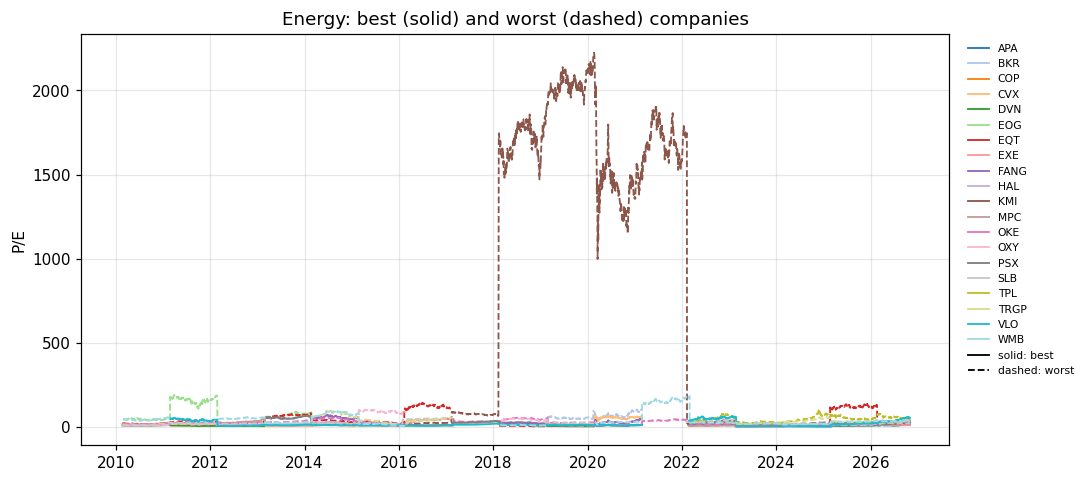
\includegraphics[width=\textwidth]{appendix/pe/energy.png}
\caption{Energy: the 10 best (solid) and worst (dashed) companies by the measure of this analysis; fund XLE.}
\end{figure}
\subsection{Health Care}
\begin{figure}[H]
\centering
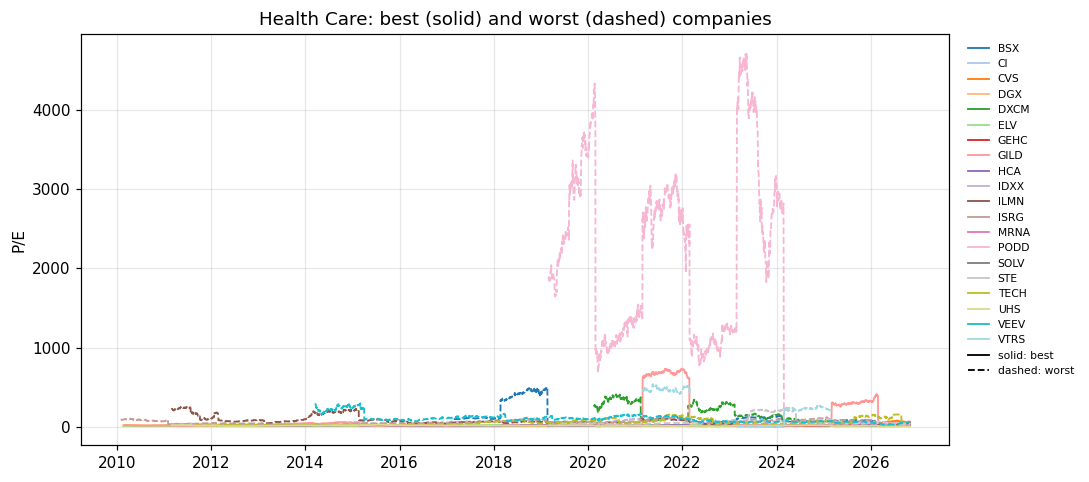
\includegraphics[width=\textwidth]{appendix/pe/health_care.png}
\caption{Health Care: the 10 best (solid) and worst (dashed) companies by the measure of this analysis; fund XLV.}
\end{figure}
\subsection{Industrials}
\begin{figure}[H]
\centering
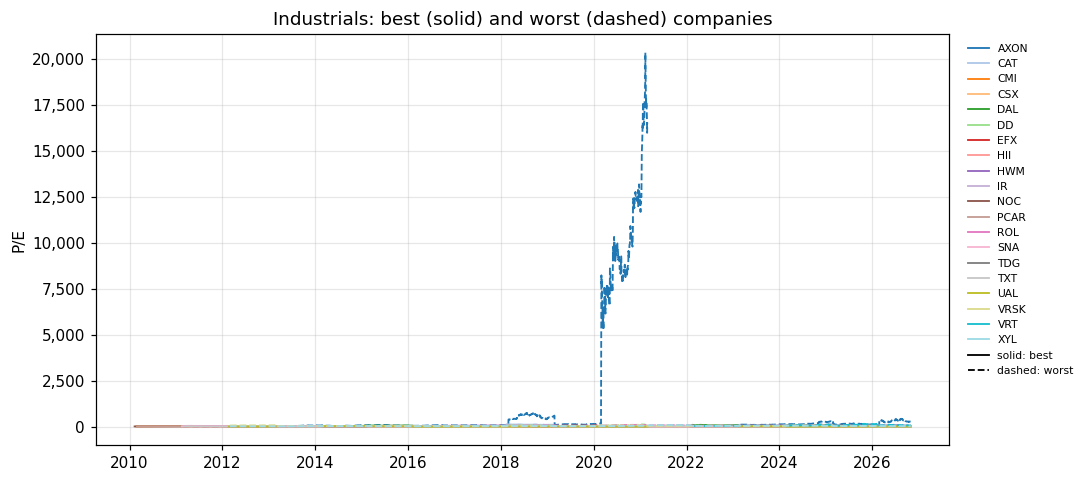
\includegraphics[width=\textwidth]{appendix/pe/industrials.png}
\caption{Industrials: the 10 best (solid) and worst (dashed) companies by the measure of this analysis; fund XLI.}
\end{figure}
\subsection{Information Technology}
\begin{figure}[H]
\centering
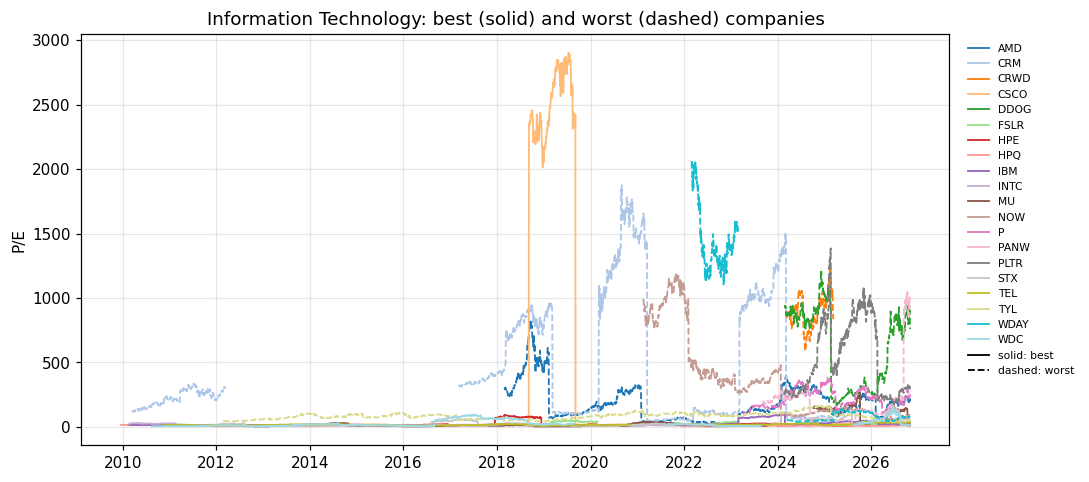
\includegraphics[width=\textwidth]{appendix/pe/information_technology.png}
\caption{Information Technology: the 10 best (solid) and worst (dashed) companies by the measure of this analysis; fund XLK.}
\end{figure}
\subsection{Materials}
\begin{figure}[H]
\centering
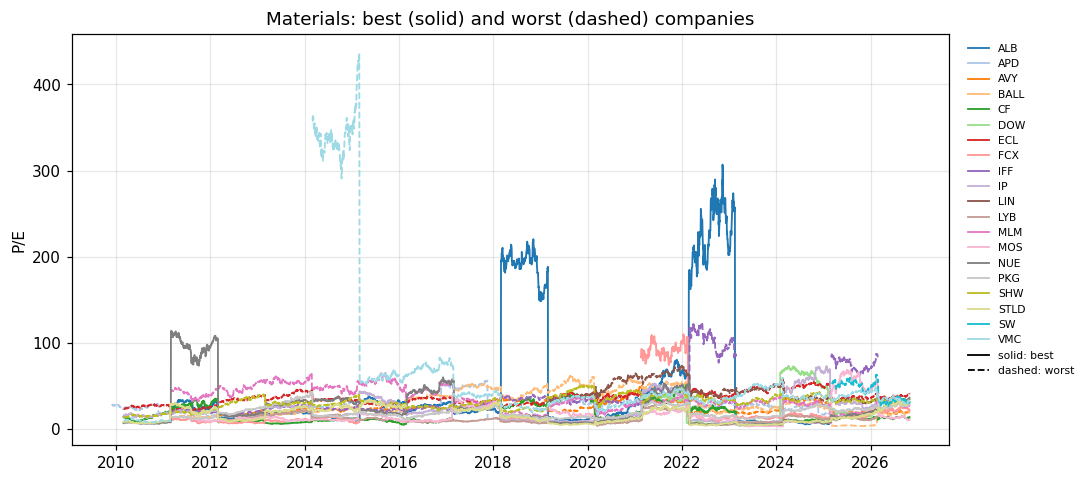
\includegraphics[width=\textwidth]{appendix/pe/materials.png}
\caption{Materials: the 10 best (solid) and worst (dashed) companies by the measure of this analysis; fund XLB.}
\end{figure}
\subsection{Utilities}
\begin{figure}[H]
\centering
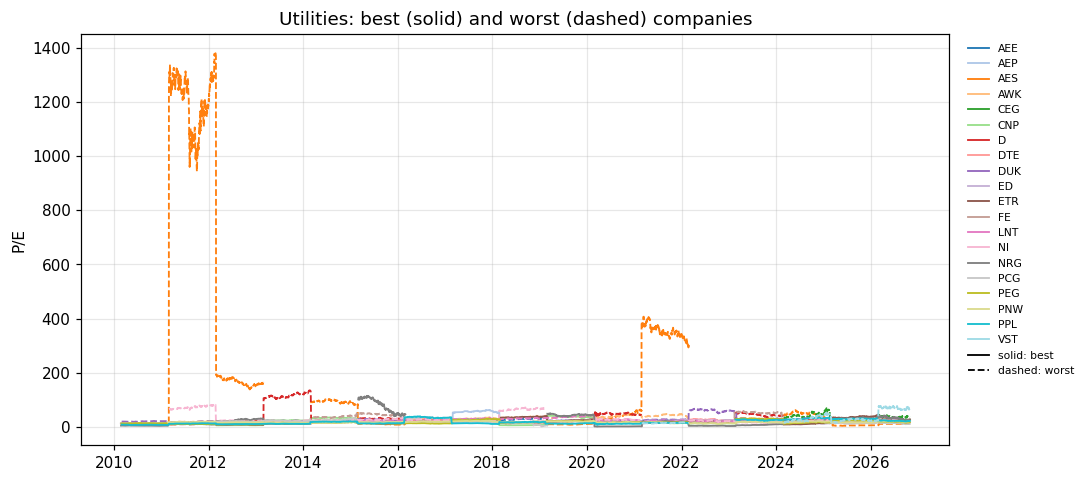
\includegraphics[width=\textwidth]{appendix/pe/utilities.png}
\caption{Utilities: the 10 best (solid) and worst (dashed) companies by the measure of this analysis; fund XLU.}
\end{figure}
\section{Dividend yield: all GICS sectors}
\label{app:dividend_yield}
For every GICS sector, its best companies (solid) against its worst (dashed) by the measure of the analysis.

\subsection{Communication Services}
\begin{figure}[H]
\centering
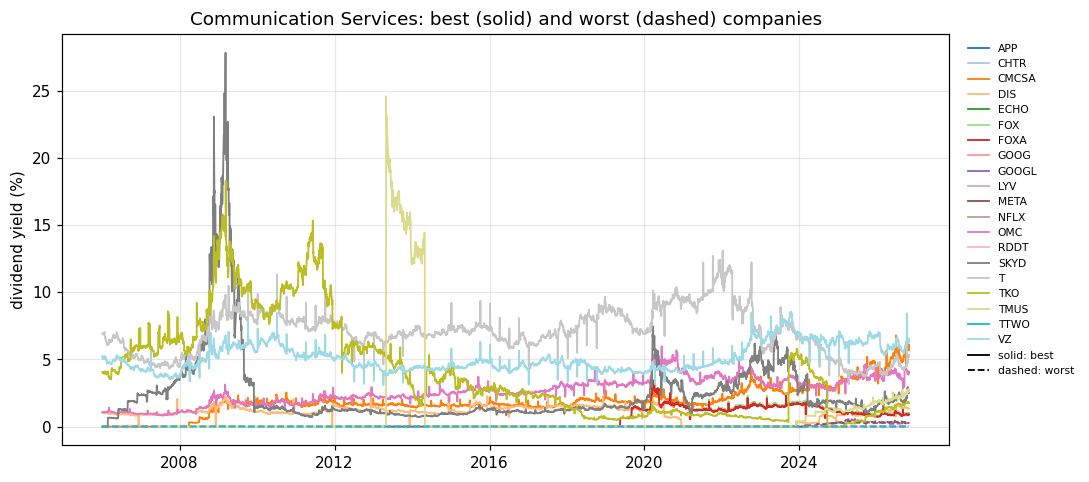
\includegraphics[width=\textwidth]{appendix/dividend_yield/communication_services.png}
\caption{Communication Services: the 10 best (solid) and worst (dashed) companies by the measure of this analysis; fund XLC.}
\end{figure}
\subsection{Consumer Discretionary}
\begin{figure}[H]
\centering
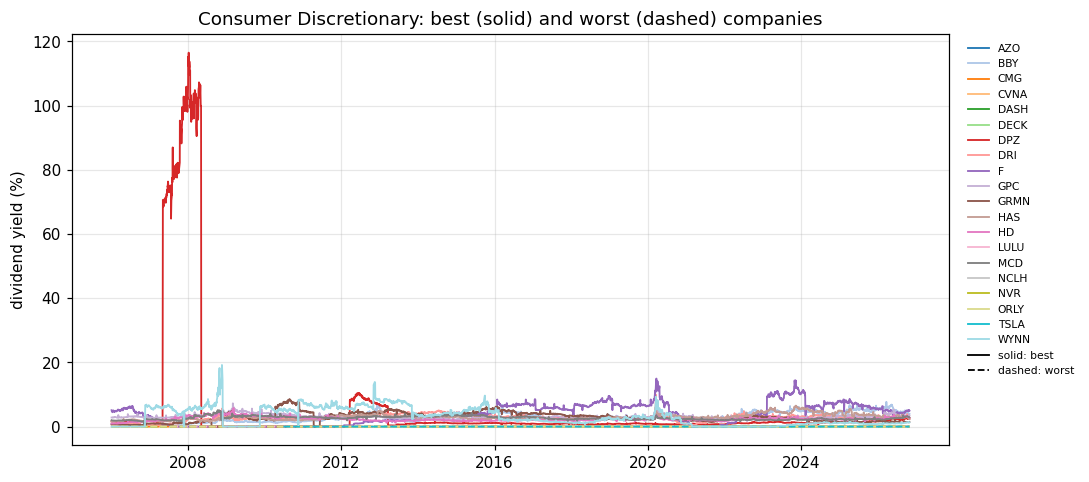
\includegraphics[width=\textwidth]{appendix/dividend_yield/consumer_discretionary.png}
\caption{Consumer Discretionary: the 10 best (solid) and worst (dashed) companies by the measure of this analysis; fund XLY.}
\end{figure}
\subsection{Consumer Staples}
\begin{figure}[H]
\centering
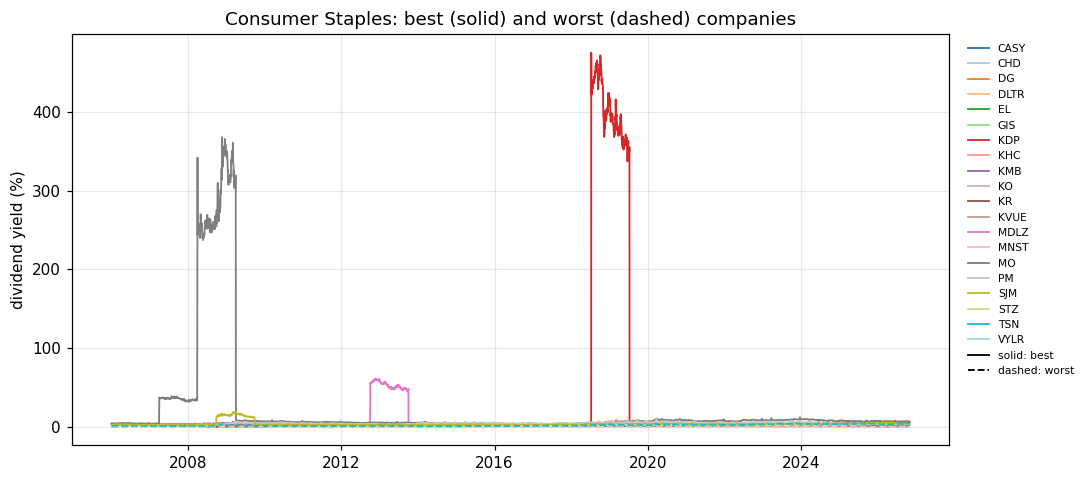
\includegraphics[width=\textwidth]{appendix/dividend_yield/consumer_staples.png}
\caption{Consumer Staples: the 10 best (solid) and worst (dashed) companies by the measure of this analysis; fund XLP.}
\end{figure}
\subsection{Energy}
\begin{figure}[H]
\centering
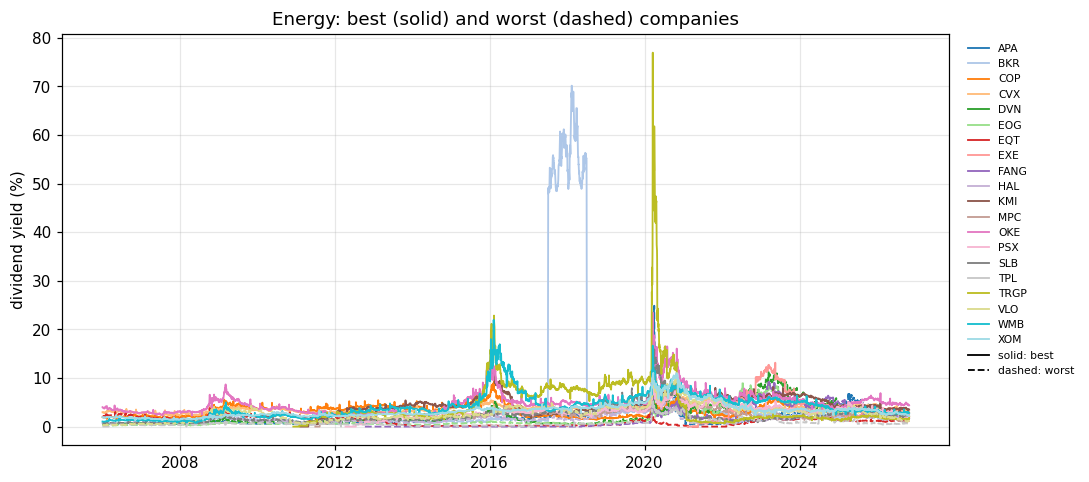
\includegraphics[width=\textwidth]{appendix/dividend_yield/energy.png}
\caption{Energy: the 10 best (solid) and worst (dashed) companies by the measure of this analysis; fund XLE.}
\end{figure}
\subsection{Health Care}
\begin{figure}[H]
\centering
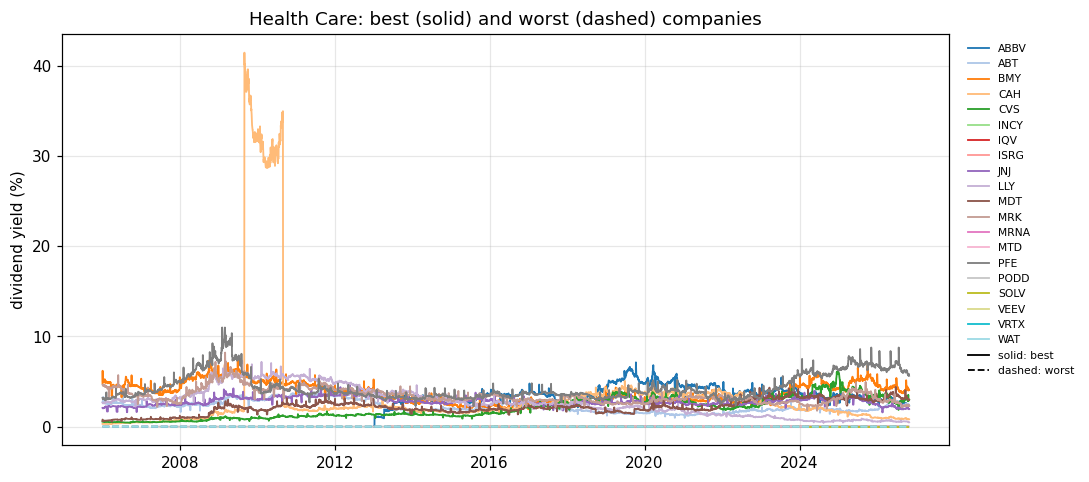
\includegraphics[width=\textwidth]{appendix/dividend_yield/health_care.png}
\caption{Health Care: the 10 best (solid) and worst (dashed) companies by the measure of this analysis; fund XLV.}
\end{figure}
\subsection{Industrials}
\begin{figure}[H]
\centering
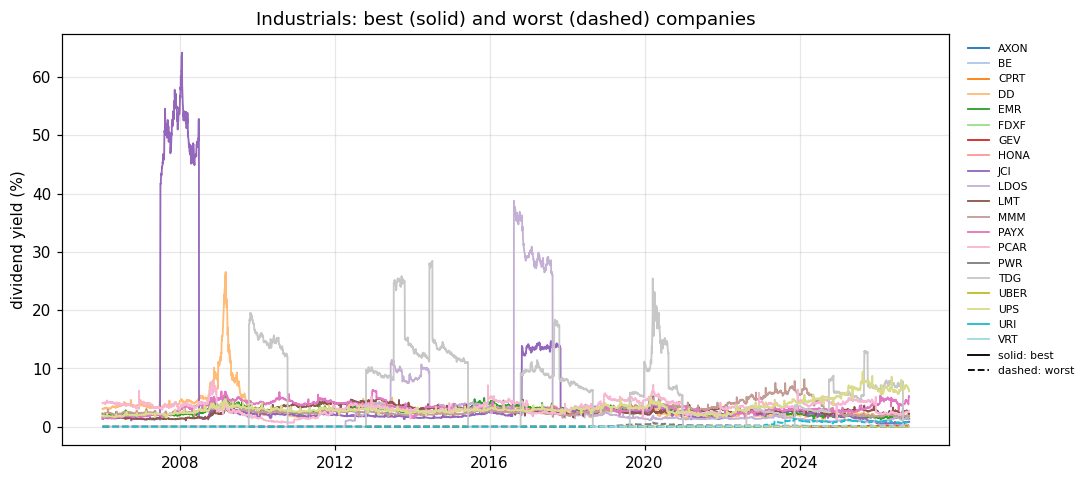
\includegraphics[width=\textwidth]{appendix/dividend_yield/industrials.png}
\caption{Industrials: the 10 best (solid) and worst (dashed) companies by the measure of this analysis; fund XLI.}
\end{figure}
\subsection{Information Technology}
\begin{figure}[H]
\centering
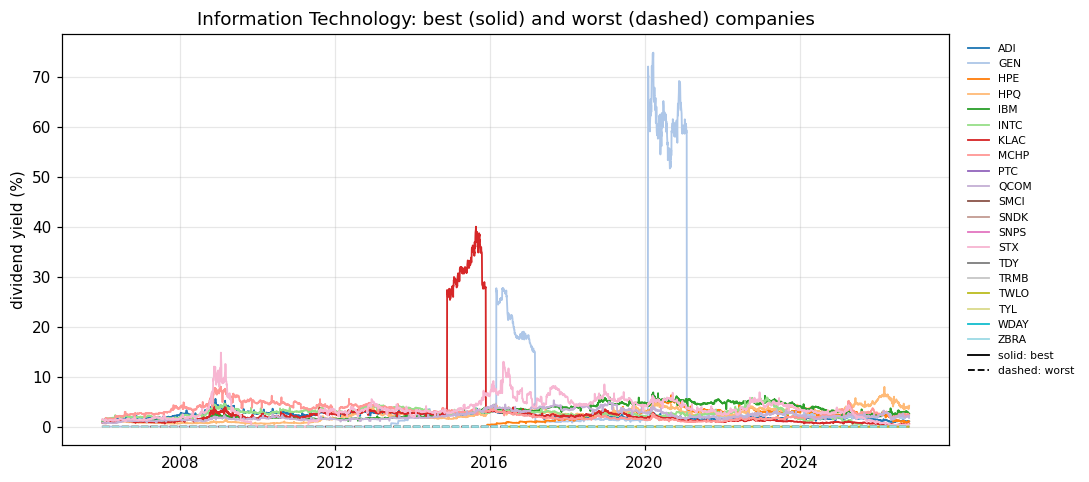
\includegraphics[width=\textwidth]{appendix/dividend_yield/information_technology.png}
\caption{Information Technology: the 10 best (solid) and worst (dashed) companies by the measure of this analysis; fund XLK.}
\end{figure}
\subsection{Materials}
\begin{figure}[H]
\centering
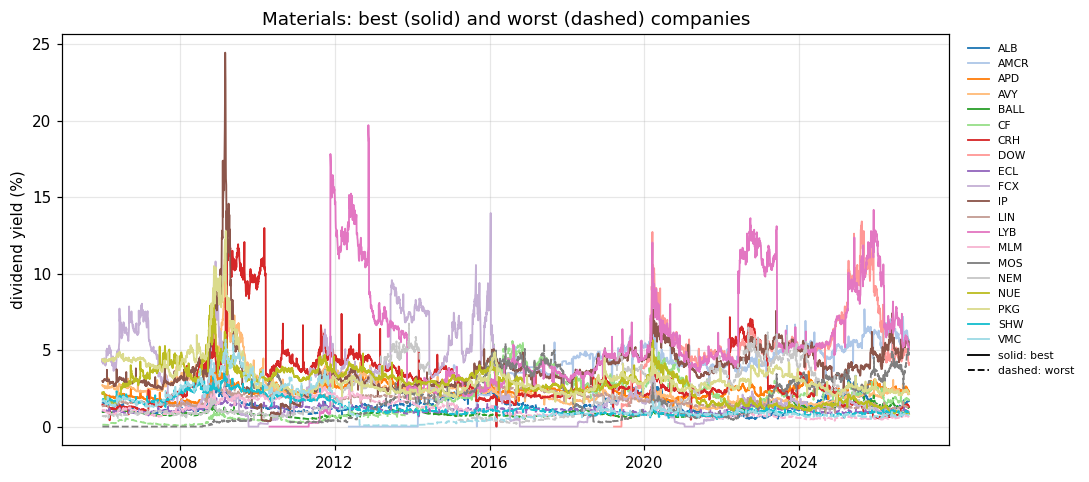
\includegraphics[width=\textwidth]{appendix/dividend_yield/materials.png}
\caption{Materials: the 10 best (solid) and worst (dashed) companies by the measure of this analysis; fund XLB.}
\end{figure}
\subsection{Utilities}
\begin{figure}[H]
\centering
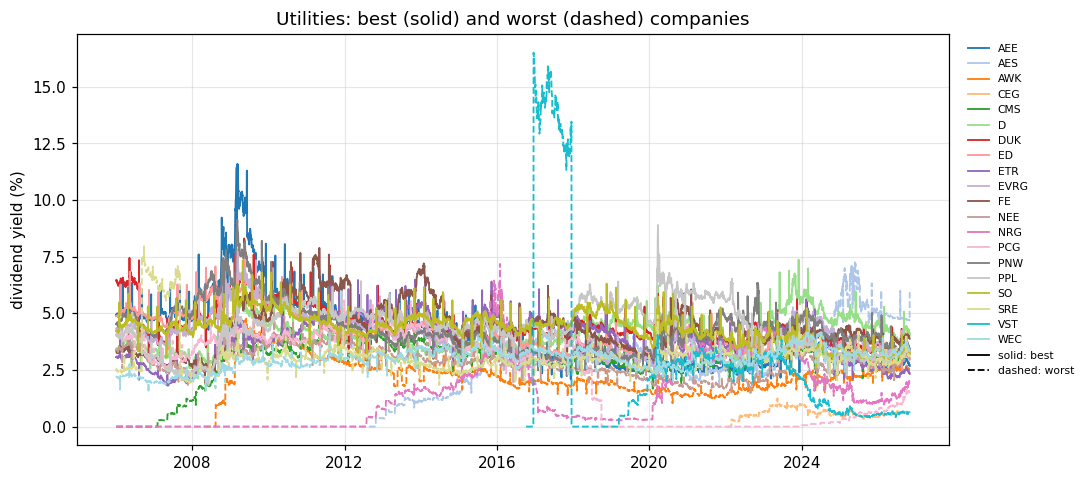
\includegraphics[width=\textwidth]{appendix/dividend_yield/utilities.png}
\caption{Utilities: the 10 best (solid) and worst (dashed) companies by the measure of this analysis; fund XLU.}
\end{figure}
\end{document}
